\documentclass[a4paper,12pt,twoside,openany]{report}

\usepackage{polski}
\usepackage{helvet}
\usepackage[T1]{fontenc}
\usepackage{anyfontsize}
\usepackage[utf8]{inputenc}
\usepackage[pdftex]{graphicx}
\usepackage{tabularx}
\usepackage{array}
\usepackage[polish]{babel}
\usepackage{subfigure}
\usepackage{amsfonts}
\usepackage{verbatim}
\usepackage{indentfirst}
\usepackage[pdftex]{hyperref}
\usepackage{amsmath}
\usepackage{float}
\usepackage{subfigure}
\usepackage{tabularx}
\usepackage{enumitem}
\usepackage{listings}
\usepackage{gensymb}

\setlist[itemize]{noitemsep, topsep=0pt}

\newcommand{\ImgPath}{.}
\newcommand{\TODO}{\textbf{TODO}}
\newcommand{\tech}{\texttt}

\def\oprawa{1.05cm}
\addtolength{\oddsidemargin}{\oprawa}
\addtolength{\evensidemargin}{-\oprawa}

\usepackage{multirow}
\usepackage{enumitem}	
\setlist{listparindent=\parindent, parsep=\parskip} 

\usepackage{prmag2017} 

\title{Rozpoznawanie gestów na przykładzie gry papier, kamień, nożyce}

\author{Adrian Szewczyk}
\nrindeksu{279074}

\opiekun{mgr inż. Marek Wdowiak}
\terminwykonania{28 stycznia 2019} 
\rok{2018}


\opinie{
  \input{opiniaopiekuna.tex}
  \newpage
  \newpage
\begin{center}
 {\large\bf  Recenzja } \\
pracy dyplomowej magisterskiej wykonanej przez dyplomanta\\
{\bf Zdolnego Studenta i Pracowitego Kolegę} \\
 Wydział Elektryczny, kierunek Informatyka,  Politechnika Warszawska\\
Temat pracy\\
\textit{\bf
TYTUŁ PRACY DYPLOMOWEJ
}\\
\end{center}
\medskip
\noindent
Recenzent: {\bf prof. nzw. dr hab. inż. Jan Surowy}\\
Ocena pracy dyplomowej: {\bf bardzo dobry}
\medskip


\centerline{\bf Treść recenzji}
   Celem pracy dyplomowej panów dolnego Studenta i Pracowitego Kolegi  było
opracowanie systemu pozwalającego symulować  i opartego o oprogramowanie o
otwartych źródłach (ang. Open Source). Jak piszą Dyplomanci, starali się opracować
system, który łatwo będzie dostosować do zmieniających się dynamicznie wymagań,
będzie miał niewielkie wymagania sprzętowe i umożliwiał dalszą łatwą rozbudowę oraz
dostosowanie go do potrzeb.
Przedstawiona do recenzji praca składa się z krótkiego wstępu jasno i
wyczerpująco opisującego oraz uzasadniającego cel pracy, trzech rozdziałów (2-4)
zawierających bardzo solidny i przejrzysty opis: istniejących podobnych
rozwiązań (rozdz. 2), komponentów rozpatrywanychjako kandydaci do
tworzonego systemu (rozdz. 3) i wreszcie zagadnień wydajności wirtualnych
rozwiązań, zwłaszcza w kontekście współpracy  kilku elementów
 sieci (rozdział 4). Piąty rozdział to opis przygotowanego przez
Dyplomantów środowiska obejmujący opis konfiguracji
środowiska oraz przykładowe ćwiczenia laboratoryjne (5 ćwiczeń). Ostatni, szósty
rozdział pracy to krótkie zakończenie, które wylicza także możliwości dalszego
rozwoju projektu. W ramach przygotowania pracy Dyplomanci zebrali i przedstawili w
bardzo przejrzysty sposób duży zasób informacji o narzędziach, Rozdziały 2, 3 i 4 świadczą o dobrej orientacji
w nowoczesnej i ciągle intensywnie rozwijanej tematyce stanowiącej
zakres pracy i o umiejętności syntetycznego, przejrzystego przedstawienia tych
wyników. Drobne  mankamenty tej części pracy to zbyt skrótowe omawianie
niektórych zagadnień technicznych, zakładające dużą początkową wiedzę czytelnika
i dość niestaranne podejście do powołań na źródła.
Utrudnia to w pewnym stopniu czytanie pracy i zmniejsza jej wartość dydaktyczną
(a ta zdaje się być jednym z celów Autorów), ale jest zrekompensowane zawartością
merytoryczną. Praca zawiera dwa dodatki, z których pierwszy obejmuje wyniki
eksperymentów i badań nad wydajnością, a drugi to źródła
skryptów budujących środowisko. Praca
zawiera niestety dość dużą liczbę drobnych błędów redakcyjnych, ale nie wpływają
one w sposób istotny na na jej czytelność i wartość. W całej pracy przewijają
się samodzielne, zdecydowane wnioski Autorów, które są wynikiem własnych i
oryginalnych badań.  Rozdział 5 i dodatki pracy przekonują mnie, że Dyplomanci dość
dobrze zrealizowali postawione przed nimi zadanie. Pozwala to stwierdzić, że
wykazali się więc także umiejętnością zastosowania w praktyce wiedzy
przedstawionej w rozdziałach 2-4. Kończący pracę rozdział szósty świadczy o
dużym (ale moim zdaniem uzasadnionym) poczuciu własnej wartości i jest
świadectwem własnego, oryginalnego spojrzenia na tematykę przedstawioną w pracy
dyplomowej. Uważam, że cele postawione w założeniach pracy zostały pomyślnie
zrealizowane. Proponuję ocenę bardzo dobrą (5).

\vskip 1cm
{
\raggedleft
(data, podpis)\kern1cm

}
}

\streszczenia{
  \newpage
\begin{center}
\large \bf
Rozpoznawanie gestów na przykładzie gry papier, kamień, nożyce
\end{center}

\section*{Streszczenie}
W pracy inżynierskiej zostało przedstawione podejście do problemu rozpoznawania gestów przez wszystkie jego etapy. W pierwszym etapie został przedstawiony zakres i cel pracy. Kolejne dwa rozdziały to teoretyczny wstęp do zagadnień oraz wykorzystanych narzędzi w pracy. 

Rozdział ,,rozwiązywanie problemu'' pokazuje podejście do klasyfikacji gestów na przykładzie gry papier, kamień, nożyce. Obrazuje aktywizację oraz  przetwarzanie danych w celu uzyskania jak najlepszego zbioru danych. W późniejszej części zostały opisane etapy filtracji, segmentacji dłoni. Po uzyskaniu zbioru danych zostały stworzone klasyfikatory. Pierwszym podejściem było stworzenie klasyfikatora KNN, a następnie stworzenie klasyfikatora bazującego na sieciach neuronowych. 

Zakończenie pracy to podsumowanie wykonanej pracy, porównanie wyników uzyskanych przez użyte klasyfikatory oraz opisanie wniosków zaobserwowanych podczas wykonywania pracy inżynierskiej.

\bigskip
{\noindent\bf Słowa kluczowe:} rozpoznawanie gestów, klasyfikacja, sieci neuronowe, OpenCV, TensorFlow, Keras, klasyfikator KNN

\vskip 2cm


\begin{center}
\large \bf
ENG Rozpoznawanie gestów na przykładzie gry papier, kamień, nożyce
\end{center}

\section*{Abstract}

\bigskip
{\noindent\bf Keywords:} ENG rozpoznawanie gestów, klasyfikacja, python, sieci neuronowe

\vfill
}

\begin{document}
\maketitle


\chapter{Wstęp}
\section{Wprowadzenie}
Istotną rolę w życiu społecznym pełnią gesty. Dodatkowa mowa niewerbowana może przekazać zdecydowanie więcej informacji niż tylko słowa wypowiedziane przez nadawcę. Gesty zazwyczaj służą do uzupełnienia mowy, do wspomożenia lub wzmocnienia przekazywanej wiadomości\cite{Collins}. W języku migowym, który pozwala na wzajemną komunikację ludzi głuchych, gesty pełnią rolę głównego medium komunikacyjnego. Oprócz samej mowy gesty mają też inne zastosowania. Przykładem takim może być gra papier, kamień, nożyce. W której każdy z graczy pokazuje jeden z trzech dostępnym gestów. W zależności od kombinacji gestów pokazanych przez graczy określany jest zwycięzca.

Interakcje człowiek-komputer są przedmiotem zainteresowania nauk na styku informatyki, nauk społecznych oraz projektowania technicznego i artystycznego. Interakcje pomiędzy użytkownikiem a komputer mają miejsce za pomocą interfejsów użytkownika, do których możemy zaliczyć zarówno sprzęt jak i oprogramowanie\cite{Kostkiewicz}. Szczególnym przypadkiem są interfejsy kinetyczne, których celem jest wykorzystywanie gestów ludzkich do interakcji człowiek-komputer. Dąży się do upodobnienia interakcji człowiek-komputer do interakcji między ludzkich. Uczymy zatem komputery, rozpoznawania gestów i mowy, tak aby komunikacja z komputerem odbywała się w sposób bardziej naturalny.

Klasyfikacja gestów jest powszechnym problem przetwarzania obrazów. Jest to temat obszerny i coraz lepiej zbadany. Klasyfikacja gestów ma szerokie zastosowanie. Jedną z zalet rozpoznawania gestów jest możliwość sterowania naszym smartfonem za pomocą ruchu rąk. Po wykonaniu gestu, a następnie po rozpoznaniu go przez  oprogramowanie telefonu wykonywana jest określona akcja. Innym wykorzystaniem klasyfikacji gestów jest sterowanie gier, gdzie jako przykład można podać urządzenie Kinect używane jako sensor dla konsoli Xbox 360\cite{Kinect}.

\section{Cel pracy}
W swojej pracy dyplomowej będę chciał przedstawić sposób podejścia do problemu klasyfikacji gestów, a następnie zaimplementować w języku Python, przy użyciu bibliotek OpenCV, TensorFlow oraz Keras działającego rozwiązania i wykorzystać go w praktyce na przykładzie gry papier, kamień, nożyce. Ogólnym celem będzie stworzenie klasyfikatora, który pozwoli na~automatyczne rozpoznawanie gestów, które są wykonywane podczas gry.

\section{Gra papier, kamień, nożyce}
Jest to klasyczna gra towarzyska, w tradycyjnym wariancie przeznaczona dla dwóch graczy. W każdej rundzie gracze pokazują gesty przez siebie wybrane z trzech dostępnych. Wszystkie rundy odbywają się na ustalony wcześniej sygnał, a pokazywane gesty powinny być jak najbardziej zsynchronizowane. Gra kończy się wtedy, jeżeli jeden z graczy osiągnie określoną wcześniej ilość zwycięstw \cite{Fisher}.


\paragraph{Trzy gesty dozwolone w grze:}
\begin{itemize} 
	\item Papier
	\item Kamień
	\item Nożyce
\end{itemize} 

\begin{figure}[H]
	\centering
	\subfigure[Gest papieru]
	{\label{fig:a}\includegraphics[width=0.3\textwidth]{\ImgPath/rys/gesty_gry/papier.png}}
	\subfigure[Gest kamienia]
	{\label{fig:b}\includegraphics[width=0.3\textwidth]{\ImgPath/rys/gesty_gry/kamien.png}}
	\subfigure[Gest nożyc]
	{\label{fig:b}\includegraphics[width=0.3\textwidth]{\ImgPath/rys/gesty_gry/nozyce.png}}
	\caption{Gesty papieru, kamienia, nożyce}
\end{figure}

Zwycięzca w danej rundzie określany jest w zależności od kombinacji gestów pokazanych przez graczy. Jeżeli obaj gracze pokazali ten sam gest, wówczas następuje remis. 

\paragraph{W przypadku kombinacji:}
\begin{itemize} 
	\item papier-kamień - zwycięzcą zostaje gracz, który pokazał gest papieru
	\item papier-nożyce - zwycięzcą zostaje gracz, który pokazał gest nożyc
	\item kamień-nożyce - zwycięzcą zostaje gracz, który pokazał gest kamienia
\end{itemize} 
\mbox{} \\	
Zachowując takie zasady, każdy z gestów ma takie samo prawdopodobieństwo zwycięstwa. W grze liczy się w dużej mierze szczęście, ale także umiejętność przewidywania gestów przeciwnika.

\chapter{Wprowadzenie teoretyczne}
\section{Obrazy cyfrowe}
\textbf{Obrazem cyfrowym f} nazywamy odwzorowanie dyskretne: 
\begin{equation}
	 \textbf{f} \colon D \to W  
\end{equation}
przy czym D jest dziedziną obrazu - skończonym zbiorem współrzędnych, a W jest jego przeciwdziedziną - zbiorem wartości \cite{Iwanowski}. W związku z dyskretną reprezentacją obrazu \textit{funkcję obrazu} można określać pojęciem \textit{macierzy obrazu}.

Dziedzina D jest iloczynem kartezjańskim skończonych zbiorów pojedynczych współrzędnych:
\begin{equation}
	 D = D_{1} \times D_{2}  \times \ldots  \times D_{n} 
\end{equation}
gdzie n jest rozmiarem przestrzeni obrazu, a $ D_{i} $ jest zbiorem wartości i-tej współrzędnej punktu obrazu. 

Przeciwdziedzina W jest również iloczynem kartezjańskim:
\begin{equation}
	 W = W_{1} \times W_{2}  \times \ldots  \times W_{n} 
\end{equation}

Każdy ze zbiorów $ W_{i} $ w zależności od rodzaju obrazu może być podzbiorem zbioru liczb naturalnych, całkowitych lub liczb rzeczywistych.

\textbf{Obrazy dwuwymiarowe} są to obrazy dla których n przyjmuje wartość równą~2. Funkcja obrazu wówczas jest funkcją dwóch zmiennych \textbf{f}(x,y), w której odwzorowanie ma zazwyczaj postać:
\begin{equation}
	 \textbf{f} \colon D = \{0, \ldots, x_{max}-1\} \times \{0, \ldots, y_{max}-1\} \to W  
\end{equation}

Wartość $ x_{max} $ oznacza rozmiar wzdłuż osi x, zaś wartość $ y_{max} $ rozmiar wzdłuż osi y. Punkty obrazów dwuwymiarowych nazywane są pikselami.

Obrazy które mogą przyjmować tylko jedną z dwóch wartości, wynoszących zazwyczaj 0 i 1 nazywamy \textbf{obrazami binarnymi}. Wówczas:
\begin{equation}
	 W = \{0,1\}  
\end{equation}


Obrazy takie możemy traktować jako strukturę składającą się z dwóch zbiorów punktów obrazu. Pierwszy z nich A jest zbiorem punktów ,,włączonych'', które możemy interpretować jako te znajdujące się na pierwszym planie - punkty pierwszoplanowe:
\begin{equation}
	 A = \{p \colon \textbf{f}(p) = 1\} 
\end{equation}
gdzie f jest funkcją obrazu. Drugi ze zbiór B składa się z pozostałych punktów tzw. punktów ,,wyłączonych'', które są również nazywane punktami tła:
\begin{equation}
	 B = \{p \colon \textbf{f}(p) = 0\} 
\end{equation}

\begin{figure}[H]	
	\centering
	\includegraphics[width=0.7\textwidth]{\ImgPath/rys/bin.png}
	
	\caption{Przykładowy obraz binarny dwuwymiarowy}
\end{figure}

\section{Operacje morfologiczne}
Operacje morfologiczne pozwalają na złożone czynności związane z analizą kształtu poszczególnych elementów obrazu oraz położeniem ich względem siebie. W wyniku operacji struktura obiektu na obrazie zostaje zmieniona, w~celu osiągnięcia określonych rezultatów. 
Operacje morfologiczne można zastosować dla obrazów binarnych oraz dla obrazów o wielu odcieniach szarości\cite{Malina}. Dzięki nim jesteśmy wstanie wyszczególnić interesujące nas części czy też przefiltrować nasz obraz. 

Podstawowymi operacjami morfologicznymi są: erozja, dylatacja, otwarcie oraz zamknięcie. Wymienione operacje można wykonywać sekwencyjnie, tworząc zaawansowane systemy analizy.

Operacje morfologiczne modyfikują wartości pikseli biorąc pod uwagę jego otoczenie. Liczbę punktów otoczenia określa tzw. element strukturalny, który definiuje wartości i ich rozmieszenie w otoczeniu. Posiada on jeden wyróżniony punkt, nazywany punktem centralnym, który nie musi być pikselem ,,włączonym''\cite{Iwanowski}. 

Najczęściej stosowane elementy strukturalne nazywamy elementarnymi. W ich skład wchodzi sąsiedztwo ośmiospójne, czterospójne oraz element liniowy poziomy i pionowy.

\begin{figure}[H]
	\centering
	\subfigure[]
	{\label{fig:a}\includegraphics[width=0.25\textwidth]{\ImgPath/rys/elementy_strukturalne/1.png}}
	\subfigure[]
	{\label{fig:b}\includegraphics[width=0.25\textwidth]{\ImgPath/rys/elementy_strukturalne/2.png}}
	\subfigure[]
	{\label{fig:b}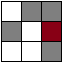
\includegraphics[width=0.25\textwidth]{\ImgPath/rys/elementy_strukturalne/3.png}}
	\caption{Dwuwymiarowy element strukturalny: (a) ośmiospójny, (b) czterospójny, (c) liniowy poziomy. Punkt w kolorze białym oznacza piksel ,,włączony'', w kolorze czarnym piksel ,,wyłączony'', a w kolorze czerwonym oznacza piksel ,,włączony'', który jest traktowany jako punkt centralny}
\end{figure}

\paragraph{Etapy przekształceń morfologicznych dla obrazów binarnych:}
\begin{enumerate}
	\item Szablon strukturalny jest przesuwany po całym obiekcie, tak aby punkt centralny znajdował się nad analizowanym pikselem
	\item Następuje porównanie otoczenia analizowanego piksela z elementem strukturalnym
	\item W zależności od stosowanej operacji morfologicznej wartość analizowanego piksela zmienia się lub też pozostaje bez zmian
\end{enumerate}

\paragraph{Erozja dla obrazów binarnych:}\mbox{} \\
\indent Erozja dla obrazów binarnych jest operacją zwężania i zmniejszania poprzez usunięcie pikseli granicznych. Usuwa wszystkie mniejsze obiekty, które możemy zinterpretować jako szumy. Definiujemy ją następująco:
\begin{equation}
	 A \ominus B = \{a \colon a + b \in A \mbox{ dla każdego } b \in B\} 
\end{equation}

\paragraph{Etapy operacji erozji:}
\begin{enumerate}
	\item Element strukturalny przesuwany jest iteracyjnie po całym obiekcie
	\item Porównuje się otoczenie analizowanego piksela z elementem strukturalnym
	\item  Jeżeli przynajmniej jeden piksel z otoczenia objętego przez szablon strukturalny ma wartość równą 0, to punkt centralny przyjmuje wartość 0. Jeżeli zaś taki przypadek nie wystąpił piksel centralny zachowuje swoją poprzednią wartość
\end{enumerate}

\begin{figure}[H]
	\centering
	\subfigure[Obraz początkowy]
		{\label{fig:a}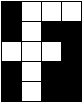
\includegraphics[width=0.35\textwidth]{\ImgPath/rys/operacje_morfologiczne/erozja_szablon.png}}
	\subfigure[Obraz wyjściowy]
		{\label{fig:b}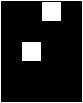
\includegraphics[width=0.35\textwidth]{\ImgPath/rys/operacje_morfologiczne/erozja2.png}}
	\caption{Operacja erozji na obrazie binarnym z elementem strukturalnym z rysunku 2.2c}
\end{figure}

\paragraph{Dylatacja dla obrazów binarnych:}\mbox{} \\
\indent Dylatacja dla obrazów binarnych jest operacją rozszerzania i zwiększania. Pozwala na wypełnienie dziur binarnych w obiektach. Jeżeli dwa obiekty są położone blisko siebie, może nastąpić złączenie w jeden obiekt. Definiujemy ją następująco: 
\begin{equation}
	 A \oplus B = \{p \colon p = a + b, a \in A, b \in B\} 
\end{equation}

\paragraph{Etapy operacji dylatacji:}
\begin{enumerate}
	\item Element strukturalny przesuwany jest iteracyjnie po całym obiekcie
	\item Następuje porównanie otoczenia analizowanego piksela z elementem strukturalnym
	\item Jeżeli przynajmniej jeden piksel z otoczenia objętego przez szablon strukturalny ma wartość równą 1, to punkt centralny przyjmuje również wartość 1. Jeżeli zaś wszystkie piksele z otoczenia piksela centralnego określonego przez element strukturalny mają wartość 0 to wówczas piksel centralny przyjmuje wartość 0.
\end{enumerate}

\begin{figure}[H]
	\centering
	\subfigure[Obraz początkowy]
	{\label{fig:a}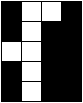
\includegraphics[width=0.35\textwidth]{\ImgPath/rys/operacje_morfologiczne/dylatacja_szablon.png}}
	\subfigure[Obraz wyjściowy]
	{\label{fig:b}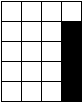
\includegraphics[width=0.35\textwidth]{\ImgPath/rys/operacje_morfologiczne/dylatacja2.png}}
	\caption{Operacja dylatacji na obrazie binarnym z elementem strukturalnym z rysunku 2.2c}
\end{figure}

\paragraph{Otwarcie dla obrazów binarnych:}\mbox{} \\
\indent Operacja otwarcia dla obrazów binarnych jest sekwencyjnym wykonaniem metod erozji oraz dylatacji. Metoda ta wygładza obiekt, usuwa pomniejsze obiekty, a w dodatku nie modyfikuje znacząco wielkości obiektów tak jak to jest w przypadku zastosowania operacji erozji czy dylatacji. Definiujemy ją następująco:
\begin{equation}
	 A \circ B = (A \ominus B) \oplus B 
\end{equation}

\paragraph{Etapy operacji otwarcia:}
\begin{enumerate}
	\item Wykonywana jest operacja erozji na zadanym obrazie
	\item Wykonywana jest operacja dylatacji na obrazie, który jest wynikiem erozji z punktu 1.
\end{enumerate}

\begin{figure}[H]
	\centering
	\subfigure[Obraz początkowy]
	{\label{fig:a}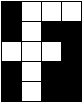
\includegraphics[width=0.32\textwidth]{\ImgPath/rys/operacje_morfologiczne/otwarcie_szablon.png}}
	\subfigure[Obraz wyjściowy]
	{\label{fig:b}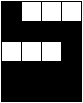
\includegraphics[width=0.32\textwidth]{\ImgPath/rys/operacje_morfologiczne/otwarcie2.png}}
	\caption{Operacja otwarcia na obrazie binarnym z elementem strukturalnym z rysunku 2.2c}
\end{figure}

\paragraph{Zamknięcie dla obrazów binarnych:}\mbox{} \\
\indent Operacja zamknięcia dla obrazów binarnych jest sekwencyjnym wykonaniem metod dylatacji oraz erozji. W rezultacie uzyskujemy połączenie obiektów o zbliżonych odległościach, wypełnienie dziur w obiektach, jednakże końcowy kształt obiektu zostaje w dużym stopniu zmieniony w stosunku do kształtu przed zastosowaniem operacji zamknięcia. Definiujemy ją następująco:
\begin{equation}
	 A \bullet B = (A \oplus B) \ominus B  
\end{equation}

\begin{figure}[H]
	\centering
	\subfigure[Obraz początkowy]
	{\label{fig:a}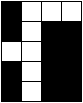
\includegraphics[width=0.32\textwidth]{\ImgPath/rys/operacje_morfologiczne/zamkniecie_szablon.png}}
	\subfigure[Obraz wyjściowy]
	{\label{fig:b}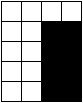
\includegraphics[width=0.32\textwidth]{\ImgPath/rys/operacje_morfologiczne/zamkniecie2.png}}
	\caption{Operacja zamknięcia na obrazie binarnym z elementem strukturalnym z rysunku 2.2c}
\end{figure}

\paragraph{Etapy operacji zamknięcia:}
\begin{enumerate}
	\item Wykonywana jest operacja dylatacji na zadanym obrazie
	\item Wykonywana jest operacja erozji na obrazie, który jest wynikiem dylatacji z punktu 1.
\end{enumerate}

\section{Filtry ruchu}
Filtry ruchu są wykorzystywane do generowania maski binarnej zawierającej poruszające się obiekty. Odejmowanie dwóch klatek z plików pozwala nam prześledzić, które z części obrazów zmieniły się. 

\begin{figure}[H]
	\centering
	\subfigure[Tło]
	{\label{fig:a}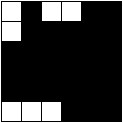
\includegraphics[width=0.3\textwidth]{\ImgPath/rys/bs/tlo.png}}
	\subfigure[Obraz binarny]
	{\label{fig:b}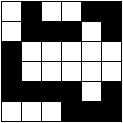
\includegraphics[width=0.3\textwidth]{\ImgPath/rys/bs/obraz.png}}
	\subfigure[Różnica]
	{\label{fig:b}\includegraphics[width=0.3\textwidth]{\ImgPath/rys/bs/bin.png}}
	\caption{Różnica obrazu binarnego oraz jego tła}
\end{figure}

Biblioteka OpenCV posiada wiele gotowych rozwiązać do wykrywania obiektów w ruchu\cite{opencvs2}. Jako przykładowe metody możemy wyróżnić następujące:
\begin{itemize} 
	\item BackgroundSubtractorMOG
	\item BackgroundSubtractorMOG2
	\item BackgroundSubtractorGMG
	\item BackgroundSubtractorKNN
	\item BackgroundSubtractorGSOC
	\item BackgroundSubtractorLSBP
\end{itemize} 
	
\paragraph{BackgroundSubtractorKNN} \mbox{} \\
 \indent
 BackgroundSubtractorKNN jest metodą segmentacji tła oraz pierwszego planu bazująca na K-najbliższych sąsiadach. Algorytm stosowany w metodzie jest bardzo wydajny, jeżeli liczba pikseli na pierwszym planie jest niska\cite{KNN}. 

\begin{figure}[H]	
	\centering
	\includegraphics[width=0.7\textwidth]{\ImgPath/rys/bs/knn.png}
	
	\caption{Przykładowy obraz po zastosowaniu metody BackgroundSubtractorKNN z biblioteki OpenCV}
\end{figure}
 
 Segmentacja oczywiście nie jest całkowicie dokładna, dlatego w celu polepszenia efektów należy zastosować dalszą filtrację. Występujące szumy są spowodowane różnymi odbiciami, cieniami czy innymi niezauważalnymi ruchami. Wówczas należy wykorzystać przedstawione wcześniej operacje morfologiczne, które poprawią nam wykonaną detekcję.

\section{Detekcja kolorów}
Celem detekcji kolorów jest wygenerowanie obrazu binarnego, w którym piksele ,,włączone'' oznaczają te, które na zadanym obrazie są w określonym przedziale kolorów. Jeżeli dany piksel nie należy do określonego  przedziału, wówczas staje się ,,wyłączony''. Detekcja taka pozwala na wyłuskanie tylko obiektów o określonej barwie.

Detekcja jest bardzo wrażliwa na różnego rodzaju szumy. Częstymi powodem występowanie ich jest zmienne oświetlenie. Obiekt przy różnym świetle możemy odbierać kolorystycznie całkowicie inaczej. W przypadku, kiedy analizujemy dynamiczny ruch, wówczas dynamika również może wpływać na kolorystykę danego obiektu.  

Aby polepszyć efekt końcowy detekcji obiektów o określonym kolorze, należy analogicznie jak w przypadku detekcji ruchu, wykorzystać odpowiednie operacje morfologiczne. 

\paragraph{Model RGB} \mbox{} \\
\indent
Model RGB składa się z trzech części: R (\textit{ang. Red}) określa wartość barwy czerwonej, G (\textit{ang. Green}) określa wartość barwy zielonej, B (\textit{ang. Blue}) określa wartość barwy niebieskiej. Wartości najczęściej są podawane w przedziale liczb całkowitych 0-255 lub w przedziale liczb rzeczywistych 0-1. Model RGB jest szeroko stosowany w urządzeniach wyświetlających obraz oraz w urządzeniach akwizycji obrazu.
\begin{figure}[H]	
	\centering
	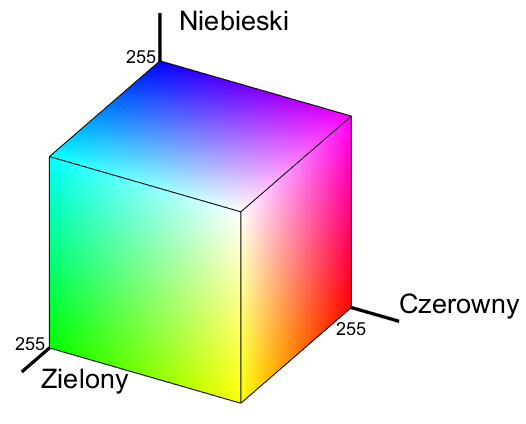
\includegraphics[width=0.62\textwidth]{\ImgPath/rys/rgb.png}
	
	\caption{Model RGB}
\end{figure}

\paragraph{Model HSV} \mbox{} \\ \indent
HSV (\textit{ang. Hue Saturation Value}) jest to model opisu przestrzeni barw, wprowadzony przez Alveya Raya Smitha w 1978 roku.

\begin{figure}[H]	
	\centering
	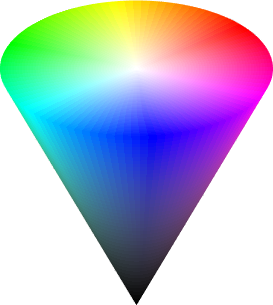
\includegraphics[width=0.42\textwidth]{\ImgPath/rys/hsv.png}
	
	\caption{Model HSV}
\end{figure}

Model składa się z następujących części: barwa, nasycenie, wartość. Geometrycznie możemy go przedstawić jako stożek. Wszystkie barwy wywodzą się ze światła białego, czyli ze środka stożka. Składowa H, oznacza barwę w postaci kąta od 0 do 360 stopni. Składowa S czyli nasycenie, geometrycznie to odległość od środka na promieniu podstawy. Decyduje o bliskości naszego koloru do koloru białego. Ostatnia składowa V, to wartość oznaczająca wysokość na stożku, którą możemy traktować jako jasność naszego koloru. Czym mniejsza jej wartość tym kolor ciemniejszy\cite{Jankowski}.

\paragraph{Konwersja z modelu RGB na model HSV: \cite{rgbhsv}} \mbox{} \\ 
\indent
Jeżeli wartość barw jest w przedziale liczb całkowitych 0-255, wówczas należy zmienić przedział na liczby rzeczywiste w zakresie 0-1: 
\begin{equation}
	 R' = R/255 
\end{equation}
\begin{equation}
	 G' = G/255 
\end{equation}
\begin{equation}
	 B' = B/255 
\end{equation}
\begin{equation}
	 C_{max} = max(R', G', B')
\end{equation}
\begin{equation} 
	 C_{min} = min(R', G', B')
\end{equation}
\begin{equation} 
	 \Delta = C_{max}-C_{min} 
\end{equation}
\begin{equation}
		H = \left\{ \begin{array}{ll}
		0 \degree & \mbox{,gdy }\Delta = 0 \\
		60 \degree * (\frac{G'-B'}{\Delta}mod6)& \mbox{,gdy }C_{max} = R' \\
		60 \degree * (\frac{B'-R'}{\Delta}+2)& \mbox{,gdy }C_{max} = G' \\
		60 \degree *  (\frac{R'-G'}{\Delta}+4)& \mbox{,gdy }C_{max} = B' \\
		\end{array} \right. 
\end{equation}
\begin{equation}
		S = \left\{ \begin{array}{ll}
		0  & \mbox{,gdy } C_{max} = 0 \\
		\frac{\Delta}{C_{max}} & \mbox{,gdy }C_{max} \neq 0 \\
		\end{array} \right. 
\end{equation}
\begin{equation}
	 V = C_{max} 
\end{equation}


\section{Klasyfikatory}
Klasyfikacja to wyznaczanie klasy decyzyjnej do której należy nowy, nieznany dotąd obiekt. Metody klasyfikacji możemy podzielić na dwie kategorie. Pierwsza z nich jest  klasyfikacją nadzorowaną, druga zaś to klasyfikacja nienadzorowana. 

Klasyfikacja nadzorowana w momencie uczenia klasyfikatora tzn. podawania zbioru danych treningowych, musi w sobie zawierać etykietę(atrybut decyzyjny), która oznacza do jakiej klasy należy ten konkretny przypadek. Zaś w przypadku ucznia nienadzorowanego atrybut decyzyjny nie istnieje.

Elementami wejścia dla stworzenia klasyfikatora jest zbiór uczący, wyjściem jest atrybut decyzyjny, oznaczający przynależność do danej klasy \cite{Malina2}.

\subsection{Klasyfikator KNN}
Klasyfikator KNN jest przykładem klasyfikacji nadzorowanej. Należy on do grupy algorytmów leniwych tzn. tych które nie tworzą wewnętrznej reprezentacji danych uczących, lecz określają rozwiązanie dopiero przy podaniu do klasyfikatora danych \cite{knn2}.

\paragraph{Po utworzeniu klasyfikatora bazującego na zbiorze uczącym, szacowanie atrybutu decyzyjnego odbywa się w następujących krokach: }
\begin{enumerate}
	\item Ustalamy wartość k
	\item Znajdujemy k obiektów treningowych, najbliższych naszemu obiektowi
	\item Analizowany obiekt należy do klasy najliczniejszej w znalezionym zbiorze z podpunktu 2
\end{enumerate}

Ocenianie odległości pomiędzy dwoma obiektami polega na umieszczaniu obiektów w przestrzeni d-wymiarowej, gdzie d opisuje ilość atrybutów dla obiektów. Metryka miary może odbywać się w różny sposób. Najczęściej jest to miara euklidesowa, jednakże możemy również wykorzystać inne miary tj. Manhattana czy Minkowskiego. 

Po znalezieniu k-najbliższych sąsiadów, atrybut decyzyjny przyjmuje wartość od najbardziej licznej klasy w wyznaczonym zbiorze.

\begin{figure}[H]	
	\centering
	\includegraphics[width=0.5\textwidth]{\ImgPath/rys/knn.png}
	
	\caption{Przykład klasyfikatora KNN dla trzech sąsiadów}
\end{figure}

Na zaprezentowanym przykładzie możemy przeanalizować działanie klasyfikatora KNN dla trzech sąsiadów. Dla wyuczonego klasyfikatora KNN próbkami, które na grafice są zaprezentowane jako kółeczka, zaś ich kolor pokazuje do jakiej klasy obiektu należą. Naszym zadaniem jest określenie atrybuty decyzyjnego dla próbki, która została zaznaczona kolorem niebieskim. W pierwszym kroku zaznaczamy najbliższe sąsiedztwo, na ilustracji zatoczono go dużym okręgiem. Można zaobserwować, że w sąsiedztwie mamy dwa obiekty klasy czerwonej oraz jeden klasy żółtej. Wybór klasy naszego obiektu jest większościowy, co oznacza, że nasza nowa, nieznana dotąd próbka danych zostanie zakwalifikowana do klasy czerwonej.


\subsection{Dobór i ocena cech}
Podstawowym elementem tworzenia klasyfikatora jest dobór odpowiednich do niego cech na których będzie bazował. Źle dobrane elementy wejścia spowodują niedokładną klasyfikację. Dlatego tak bardzo ważne jest odpowiedni dobór cech opisujących.

Istotnym etapem dla każdej cechy była jej normalizacja danych, aby dana cecha nie powodowała większego wpływu od innych czy też wpływała nieznacząco w stosunku do innych. Przykładem normalizacji jest standaryzacja, którą możemy przedstawić zgodnie ze wzorem: 
\begin{equation}
	  Z = \dfrac{x - \mu}{\sigma} 
\end{equation}
x - wartość przed normalizacją \\ $\mu$ - średnia \\ $\sigma$ - odchylenie standardowe

\paragraph{Warunki dobrej cechy diagnostycznej: }
\begin{itemize}
	\item Powinny być wielkościami z podobnego zakresu
	\item Wartości danej cechy w obrębie określonej klasy powinny być do siebie możliwie jak najbardziej zbliżone
	\item Powinny być mało wrażliwe na szum
	\item Ta sama cecha powinna przyjmować różne wartości w przypadku różnych klas
	\item Ogólna liczba cech diagnostycznych nie może być zbyt duża \cite{Osowski}
\end{itemize}
\mbox{} \\
Warunkiem dobrej cechy diagnostycznej, jest to, że ta sama cecha w obrębie różnych klas powinna przyjmować jak najbardziej różne wartości. Przy diagnostyce tego warunku można wykorzystać średnią arytmetyczną wartości danej cechy w poszczególnych klasach.

Kolejnym warunkiem na jaki warto zwrócić uwagę podczas oceny cech jest jej odchylenie standardowe w obrębie określonej klasy. Odchylenie standardowe można określić wzorem: 
\begin{equation}
	 \sigma = {\sqrt {\operatorname {E} ((X-\operatorname {E} (X))^{2})}} 
\end{equation}
X - zmienna \\
E - wartość oczekiwana 


Opisuje ono rozproszenie cechy w obrębie określonej klasy co implikuje, że dobrze dobrana cecha charakteryzuje się jak najmniejszym rozproszeniem.

\paragraph{Przykładowe cechy możliwe do wykorzystania do opisu masek binarnych: }
\begin{itemize}
	\item Stosunek szerokości do wysokości obiektu binarnego
	\item Stosunek powierzchni obiektu binarnego do powierzchni całego obrazu
	\item Stosunek powierzchni otoczki wypukłej na obiekcie binarnym do powierzchni całego obrazu
	\item Stosunek półosi małej do dużej elipsy opisanej na obiekcie binarnym 
	\item Wartości punktów końcowych obiektu binarnego
	\item Orientacja obiektu binarnego
\end{itemize}
\mbox{} \\
Przy wyborze odpowiednich cech ważnym elementem jest ich ocena, aby sprawdzić czy wybrana cecha będzie pozytywnie wpływała na klasyfikację.

\section{Sieci neuronowe}
Sieci neuronowe możemy traktować jako model czarnej skrzynki. Dla określonych danych wejściowych uzyskujemy wartości wyjściowe.

\begin{figure}[H]	
	\centering
	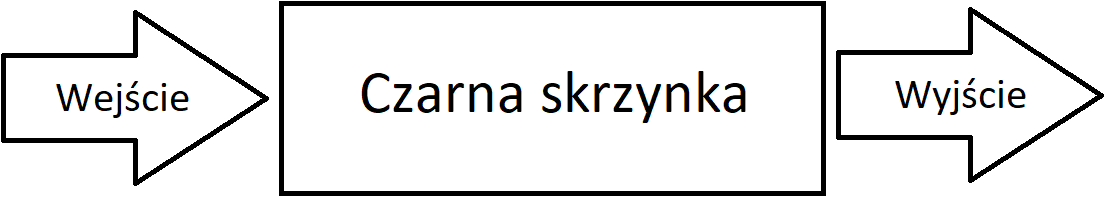
\includegraphics[width=0.95\textwidth]{\ImgPath/rys/czarna_skrzynka.png}
	
	\caption{Sieć neuronowa jako model czarnej skrzynki}
\end{figure}

Sztuczne sieci neuronowe są to systemy komputerowe zainspirowane biologiczną siecią neuronowa ludzkiego mózgu. Sieci neuronowe nie są algorytmami, jednakże są ogólnym modelem wykorzystywanym przy uczeniu maszynowym i przy przetwarzaniu danych wejściowych.

Sieci neuronowe są to zbiory połączonych ze sobą sztucznych neuronów \cite{Osowski}. W biologicznym układzie mózgu, połączenia pomiędzy dwoma neuronami nazywamy synapsami. W sztucznych sieciach neuronowych połączenie to często nazywamy krawędzią. 

Czarna skrzynka to tzw. warstwa ukryta. Znajdują się w niej neurony ściśle ze sobą powiązane. Każdy z neuronów ma w sobie pewną wartość, powszechnie oznaczaną przez wartość liczby rzeczywistej. Każda krawędź w sieciach neuronowych posiada pewną określoną wagę. Zwiększanie lub zmniejszanie wag zmienia siłę sygnału w danym połączeniu pomiędzy neuronami.

\begin{figure}[H]	
	\centering
	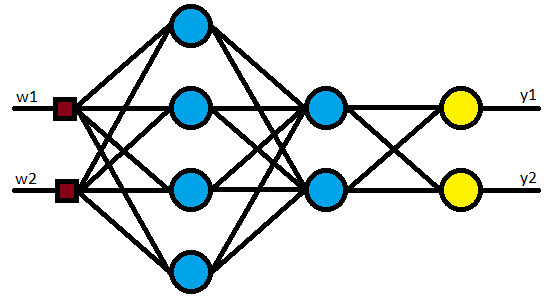
\includegraphics[width=0.70\textwidth]{\ImgPath/rys/siec_neuronowa.png}
	
	\caption{Przykładowa sieć neuronowa}
\end{figure}

Na rysunku 3.2 zaprezentowano przykładowy schemat sieci neuronowej. Sieć ta zawiera dwa elementy wejścia, które są przekazywane do każdego neuronu z pierwszej warstwy ukrytej. Model posiada dwie warstwy ukryte, które są oznaczone na modelu kolorem niebieskim. Pierwsza z nich zawiera cztery neurony, zaś druga warstwa posiada dwa neurony. Ostatnia warstwa modelu, czyli warstwa wyjściowa oznaczona kolorem żółtym posiada dwa neurony, których wyjście jest interpretowane jako rezultat działania całej sztucznej sieci neuronowej.

Sztuczne neurony na podstawie zsumowanych iloczynów wartości na wejściowych oraz wartości wag odpowiadających im krawędziom, wykonują pewną funkcję tak zwaną funkcję akwizycji, której rezultat jest traktowany jako wyjście dla pojedynczego neuronu. 

\begin{figure}[H]	
	\centering
	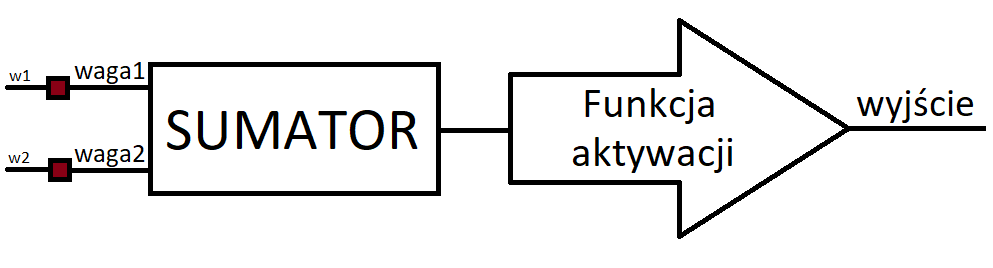
\includegraphics[width=0.95\textwidth]{\ImgPath/rys/neuron.png}
	
	\caption{Przykład pojedynczego neuronu}
\end{figure}

\paragraph{Funkcje aktywacji:}
\mbox{} \\ \indent
Wartość funkcji aktywacji dla danego neuronu, określa wartość wyjściową tego neuronu. Często używa się tej samej funkcji aktywacji dla tej samej warstwy, a niejednokrotnie wykorzystujemy tę samą funkcję aktywacji nawet do całej sieci neuronowej. 

\begin{equation}
  f(x) = max(0, ax) 
\end{equation}
\begin{figure}[H]	
	\centering
	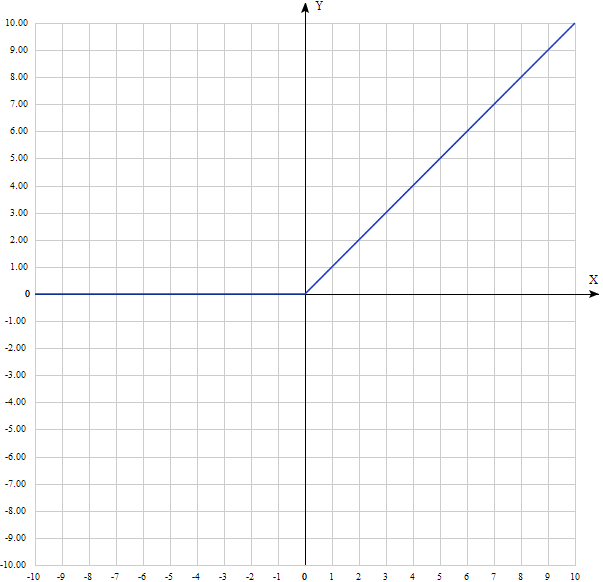
\includegraphics[width=0.65\textwidth]{\ImgPath/rys/funkcje_aktywacji/relu.png}
	
	\caption{Funkcja ReLU}
\end{figure}

\begin{equation}
  f(x) = \frac{1}{1 + exp(-\beta x)} 
\end{equation}
\begin{figure}[H]	
	\centering
	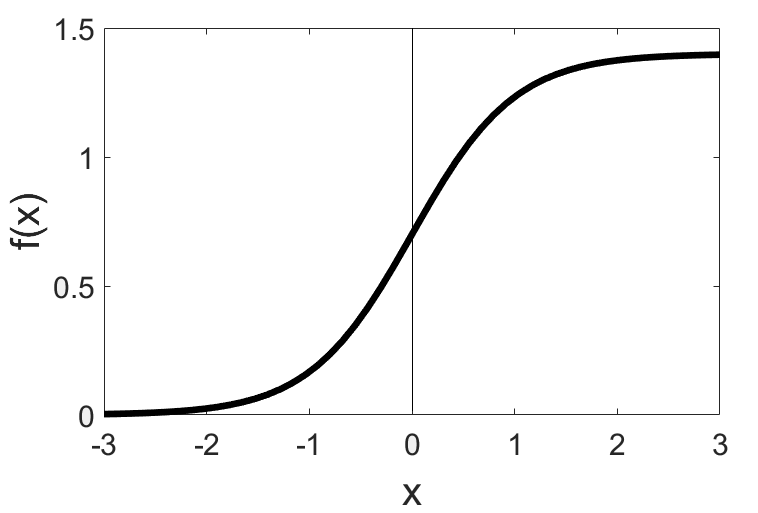
\includegraphics[width=0.65\textwidth]{\ImgPath/rys/funkcje_aktywacji/sigmoid.png}
	
	\caption{Funkcja Sigmoid}
\end{figure}


\begin{equation}
	 f(x) = tanh(\beta x) 
\end{equation}
\begin{figure}[H]	
	\centering
	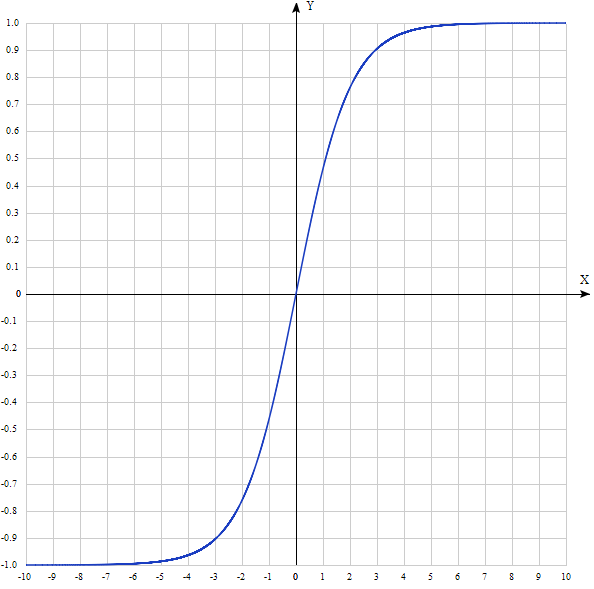
\includegraphics[width=0.65\textwidth]{\ImgPath/rys/funkcje_aktywacji/tanh.png}
	
	\caption{Funkcja Tanh}
\end{figure}

Softmax jest przykładem funkcji aktywacji, którą często wykorzystuje się jako funkcję aktywacji w warstwie wyjściowej. Suma wartości aktywacji dla całej warstwy jest równa 1. Wykorzystując tę normalizację, możemy wartości wyjściowe neuronów zinterpretować jako prawdopodobieństwo przynależności do poszczególnych klas, które reprezentowane są przez neurony wyjściowe. Funkcję Softmax definiujemy następująco: \\ 
\begin{equation}
    f(y_{i}) = \frac{exp(y_{i})}
		{\sum_{j=1}^{n} exp(y_{j})}
\end{equation}

\paragraph{Uczenie sieci neuronowych:}
\mbox{} \\
\indent
Uczenie sieci polega na dostrajaniu wartości wag poszczególnych neuronów. Przy uczeniu nadzorowanym sieci podstawowym algorytmem jest wsteczna propagacja błędu. Znając wartości wyjściowe dla danego zbioru danych wejściowych jesteśmy wstanie policzyć błąd działania sieci. Ten błąd jest przekazywany iteracyjnie do połączonych w poprzednich warstwach neuronów. Ważnym parametrem przy uczeniu sieci jest parametr szybkości uczeniu. Określa on szybkość uczenia się sieci neuronowych. 

\paragraph{Wykorzystanie sieci neuronowych:}
\begin{itemize}
	\item Rozpoznawanie obrazów
	\item Przewidywanie wartości akcji spółek giełdowych
	\item Generowanie plików wideo z obrazka
	\item Rozpoznawanie mowy
	\item Tworzenie opisu zdjęć
	\item Przewidywanie prognozy pogody
	\item Diagnostyka medyczna
	\item Ocena zdolności kredytowej
	\item Rekomendowanie reklam
\end{itemize}

\chapter{Wykorzystane narzędzia}

\section{OpenCV}
Biblioteka OpenCV (ang.\textit{ Open Source Computer Vision Library}) jest wykorzystywana przy rozpoznawaniu obrazów oraz przy uczeniu maszynowym. Została napisana w języku C przez programistów z firmy Intel w 1999 roku \cite{opencv}.

W późniejszym czasie kolejne części biblioteki były także pisane w języku C++. Biblioteka OpenCV umożliwia pisanie kodów nie tylko w językach C i C++ ale również mamy możliwość wykorzystywania tej biblioteki w językach Python, Java czy też Matlab. W związku z popularnością biblioteki udostępniono nakładki do języków takich jak C\#, Perl cz Ruby, aby móc również wykorzystywać zalety  biblioteki\cite{opencv2}. 

Biblioteka OpenCV udostępnia zaawansowaną funkcjonalność  w szeroko rozumianym pojęciu rozpoznawaniu obrazów:

\begin{itemize}
	\item przetwarzania obrazów
	\item klasyfikowaniu wzorców
	\item dokładnych pomiarów obrazów
\end{itemize}

Jako główne zalety biblioteki OpenCV możemy wyróżnić, że jest ona darmowa oraz że jest o otwartych źródłach. Zawiera bogaty zakres funkcjonalności, a kod biblioteki został napisany w sposób zoptymalizowanym, tak aby operacje wymagające dużej mocy obliczeniowej czy działające w czasie rzeczywistym mogły wykonywać się możliwie jak najszybciej.

Biblioteka OpenCV od 20 lat znajduje zastosowanie w wielu dziedzinach naszego codziennego życia:
\begin{itemize} 
	\item medycyna
	\item robotyka
	\item samochody autonomiczne
	\item systemy antywłamaniowe 
	\item systemy zabezpieczające
	\item rozpoznawanie gestów
	\item segmentacja obiektów
	\item wykrywanie ruchu
	\item rozszerzona rzeczywistość
	\item rozpoznawanie obiektów
\end{itemize}

\section{Python}
Jest to interpretowany, obiektowy język wysokiego poziomu. Używany jest w szerokiej gamie  aplikacji. Jest językiem ogólnego przeznaczenia, co oznacza, że może zostać wykorzystany praktycznie do wszystkiego. Jest rozwijany jako projekt o otwartych źródłach. Pojawił się w roku 1991, zaprojektowany przez holenderskiego programistę Guido van Rossum\cite{python1}.  

\paragraph{Zalety używania Pythona:}
\begin{itemize} 
	\item prosta, czytelna, klarowna składnia, zmniejszająca ilość potrzebnych linijek kodu w programach
	\item dynamicznie zarządza pamięcią oraz typy danych
	\item nie wymusza stylu programowania
	\item jest wieloplatformowy
	\item posiada bogaty zbiór różnego rodzaju bibliotek
	\item łatwy do nauczenia, nawet dla osób zaczynających programować
	\item szybkość działania w stosunku do innych języków skryptowych\cite{python}
\end{itemize} 
\mbox{} \\
Jeśli mielibyśmy dyskutować o wadach językach Python to ciężko jednoznacznie wskazać takie. Na pewno część z programistów może uznać zalety dynamicznego zarządzania typami jako wadę, ponieważ w niektórych przypadkach może spowodować błędy trudniejsze do znalezienia. Działania Pythona jest również wolniejsze w stosunku do języków takich jak C czy C++.  Za jedną z wad na pewno można uznać sposób programowania obiektowego jakie odbywa się w Pythonie. W szczególności nie ma enkapsulacji, istnieją metody które symulują takie działa, jednakże w stosunku do innych języków  obiektowych czytelność kodu zdecydowanie jest zmniejszona.

Język mimo swoich lat ciągle zyskuje na popularności. Ostatnio wszedł do pierwszej trójki najbardziej popularnych języków programowania według TIOBE\footnote{stan na styczeń 2019}\cite{tiobe}, wyprzedzając między innymi język C++, a ulegając jedynie językowi Java oraz C. Wzrost języka Python na pewno można łączyć ze wzrostem popularności uczenia maszynowego i głębokich sieci, gdzie język Python jest jednym z najlepszych, jak nie najlepszym językiem w tych dziedzinach. Bardzo bogata biblioteka oraz przyjemna składnia sprawia, że język Python jest częściej wykorzystywany.  

Jako ciekawostkę można powiedzieć, że nazwa języka Python wzięła się nie od zwierzęcia, lecz od słynnego Brytyjskiego serialu ,,Monty Python’s Flying Circus''\cite{python1}.

\section{TensorFlow}
Jest to biblioteka programistyczna wykorzystywana w uczeniu maszynowym i głębokich sieciach neuronowych. Została wydana jako otwarte oprogramowanie przez Google Brain Team w dniu 9 listopada 2015\cite{tensorflow}.

Umożliwia pisanie programów m.in. w językach takich jak Python czy C. Jest dostępny na 64-bitowych systemach operacyjnych: Windows, Linux, macOS oraz na platformach mobilnych: Android oraz iOS. Zaś w maju 2017 został wydany TensorFlow Lite jako dedykowane rozwiązanie specjalnie dla użytkowników Androida\cite{tensorflowlite}.

Olbrzymią zaletą biblioteki TensorFlow jest to, że reprezentuje on paradygmat Dataflow, w którym program ma postać grafu skierowanego modelującego przepływ danych pomiędzy niezależnymi operacjami w węzłach. W pierwszym kroku należy zdefiniować model, a następnie stworzyć tzw. TensorFlow session, która pozwala na uruchomienie programu. Takie podejście do pisania programów posiada ogromną zaletę jaką jest możliwość efektywnego programowania równoległego oraz rozproszonego\cite{tensorflowG}. 

TensorFlow daje możliwość nie tylko wykorzystania mocy obliczeniowej procesora, ale równie dobrze korzystania z mocy kart graficznych. Wszystko to powoduje pełne wykorzystanie komputerów przy obliczeniach równoległych.

TensorFlow oprócz niskopoziomowych struktur posiada również moduły wyższego poziomu. Do modułów niskiego poziomu możemy odwoływać się poprzez warstwę API, która umożliwia łatwy do używania interfejs przeznaczony do modelów głębokiego uczenia. Zaś nad warstwą API znajduje się warstwa wysokiego poziomu.

\section{Keras}
Biblioteka Keras została napisana w języku Python i wydana w marcu 2015 przez pierwotnego autora François Chollet\cite{keras}. 

Jej głównym przeznaczeniem jest to, aby w jak najprostszy i  jak najszybszy sposób umożliwić pracę w głębokich sieciach neuronowych. Biblioteka została zaprojektowana w sposób przyjemny do użytkowania, skupiona na modularności oraz rozszerzalności. Zaś od 2017 roku TensorFlow wspiera bibliotekę Keras. Dzięki czemu Keras jest wysokopoziomową warstwą tworzenia modelów sieci neuronowych i jej uczenia w bibliotece TensorFlow.

\chapter{Rozwiązanie problemu}
\section{Akwizycja danych}
Pierwszym etapem mojej pracy była akwizycja danych potrzebnych do uczenia maszynowego. Zbieranie danych polegało na nagrywaniu plików wideo, na których dana osoba wykonywała określony gest. W swojej pracy dyplomowej zakładałem, że każdy wykonywany gest, jest pokazywany w niebieskiej rękawiczce. To założenie wykorzystywałem w całej swojej pracy inżynierskiej.

\begin{figure}[H]	
	\centering
	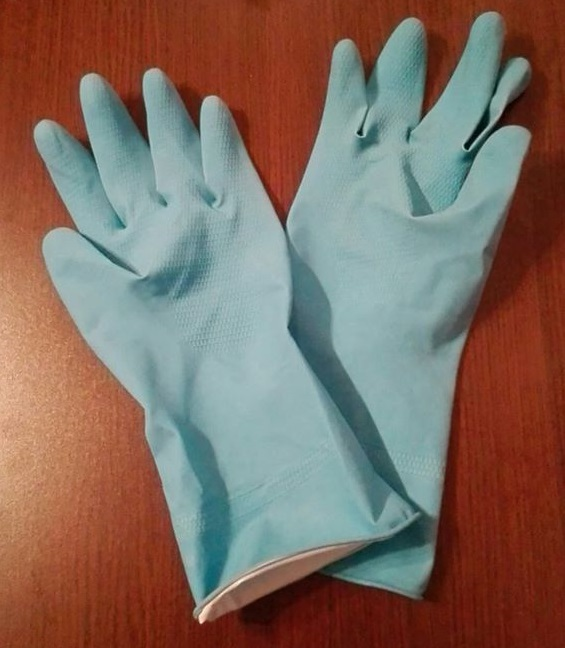
\includegraphics[width=0.37\textwidth]{\ImgPath/rys/rekawiczki.jpg}
	
	\caption{Rękawiczki wykorzystywane w pracy inżynierskiej}
\end{figure}

Osoba podczas nagrywania wykonuje ciąg określonych gestów, w dowolnym odstępie czasu. Jest ona ustawiona prostopadle do kamery, co pozwala, aby gest odbywał się poprzez wyciągnięcie ręki oraz jego pokazanie. Na nagraniu zostaje zarejestrowany wykonywany gest, tak aby jedyną widoczną częścią ciała była prawa dłoń oraz ewentualnie cześć przedramienia. 

\begin{figure}[H]	
	\centering
	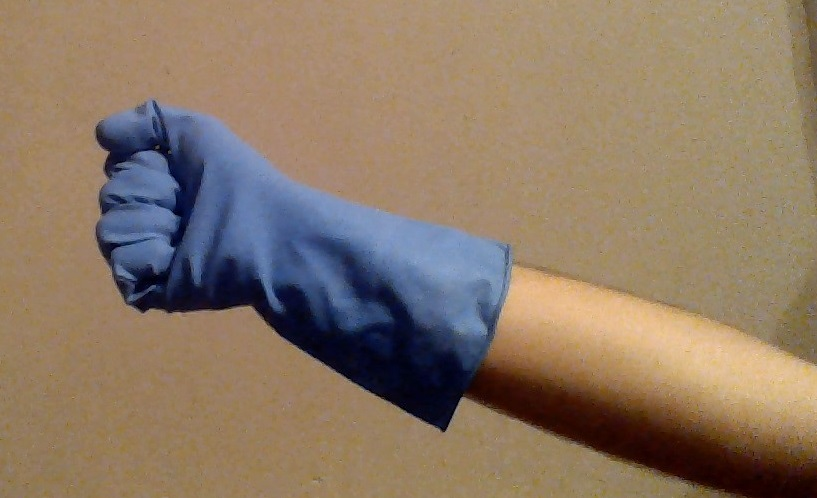
\includegraphics[width=0.45\textwidth]{\ImgPath/rys/klatka.jpg}
	
	\caption{Przykładowa klatka z nagrania}
\end{figure}

\paragraph{Do nagrywania plików wideo używałem dwóch kamer dedykowanych w laptopach:}
\begin{itemize}
	\item USB2.0 UVC HD Webcam
	\item HD Webcam
\end{itemize}
\mbox{} \\

Obie kamery przy dostatecznie dobrym oświetleniu pozwoliły na zadowalające efekty zbierania danych. Klatki plików wideo były w rozdzielczości 1280x720, co pozwoliło, że jakość nagrań była bardzo zadowalająca, pozwalająca bez problem rozpoznawać wykonywany gest. 

Również liczba klatek na sekundę umożliwiła, aby dynamiczny ruch był płynny i łatwy do prawidłowego wysegmentowania. Pierwsza kamera zapewniła 7.49 klatek na sekundę, druga zaś 16.46 klatek na sekundę.
 
W celu zebrania jak najszerszego zakresu danych, zbieranie gestów nie ograniczyło się do jednej osoby, jednakże do pięciu różnych osób:
\begin{itemize}
	\item trzech kobiet
	\item dwóch mężczyzn
\end{itemize}
\mbox{} \\
\indent 
 Zbieranie danych na różnych osobach pozwala na zmniejszenie wpływu charakterystycznych cech dla danej osoby. 
\begin{itemize}
	\item długości dłoni
	\item szerokości dłoni
	\item ułożenia palców
	\item nachylenia dłoni
\end{itemize}
\mbox{} \\
\indent
Tak zebrane dane dają ogólny pogląd na różnorodność cech danego gestu. Sprawia, że uczenie maszynowe jest skuteczniejsze i daje oczekiwane rezultaty. 

Po zgromadzeniu całego materiału wideo przeszedłem do etapu wyznaczania numerów klatek nagrań, na których był widoczny moment wykonanego gestu. Informacje o numerach klatek nagrania wykorzystywałem w późniejszym etapie, przy segmentacji dłoni z wykonanym gestem.

\paragraph{W mojej pracy inżynierskiej wykorzystywałem zbiór danych składający się z:}
\begin{itemize}
	\item 350 próbek gestu papieru
	\item 350 próbek gestu kamienia
	\item 350 próbek gestu nożyc
\end{itemize}
 Zbiór danych był równomiernie rozłożony na 5 osób - po 70 próbek na każdy gest jednej osoby.
 
 Aby zapewnić prawidłowe rozpoznawanie, należy zgromadzić jak największą liczbę próbek gestów, która będzie w późniejszych etapach wykorzystywana przy uczeniu oraz weryfikacji klasyfikatorów.

\section{Detekcja ruchu}
Po zebraniu danych zająłem się ich przetwarzaniem. Pierwszym krokiem było wysegmentowanie obiektów, które znajdowały się w ruchu. Aby to osiągnąć, należało wygenerować maskę binarną, która rozdziela elementy obrazu, która są w ruchu, od tych, które są elementami statycznymi. Do tego wykorzystałem usuwanie tła przez odejmowanie klatek realizowane przez metody \textit{BackgroundSubtractor} z biblioteki OpenCV.

W swojej pracy inżynierskiej w analizie wziąłem pod uwagę następujące dostępne funkcje:

\begin{itemize} 
	\item BackgroundSubtractorMOG
	\item BackgroundSubtractorMOG2
	\item BackgroundSubtractorGMG
	\item BackgroundSubtractorKNN
	\item BackgroundSubtractorGSOC
	\item BackgroundSubtractorLSBP
\end{itemize} 

\begin{figure}[H]
	\centering
	\subfigure[BackgroundSubtractorKNN]
	{\label{fig:a}\includegraphics[width=0.28\textwidth]{\ImgPath/rys/bs/knn.png}}
	\subfigure[BackgroundSubtractorGSOC]
	{\label{fig:b}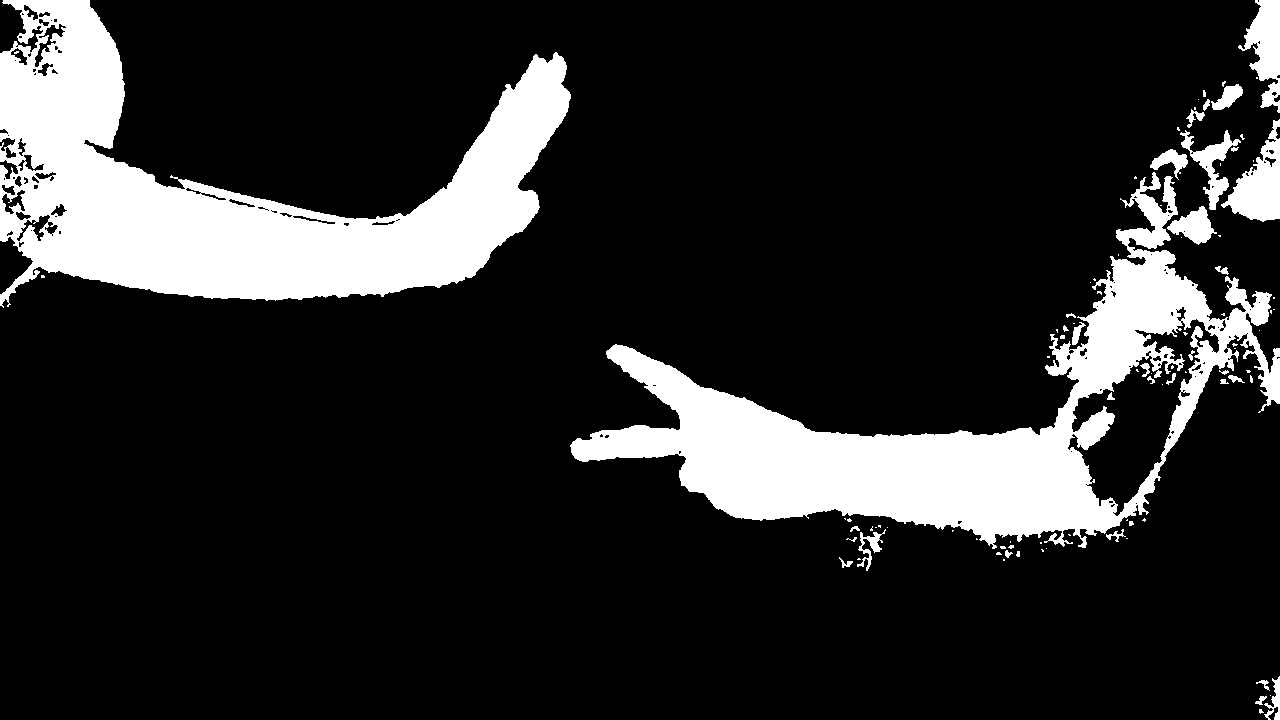
\includegraphics[width=0.28\textwidth]{\ImgPath/rys/bs/gsoc.png}}
	\subfigure[BackgroundSubtractorLSBP]
	{\label{fig:b}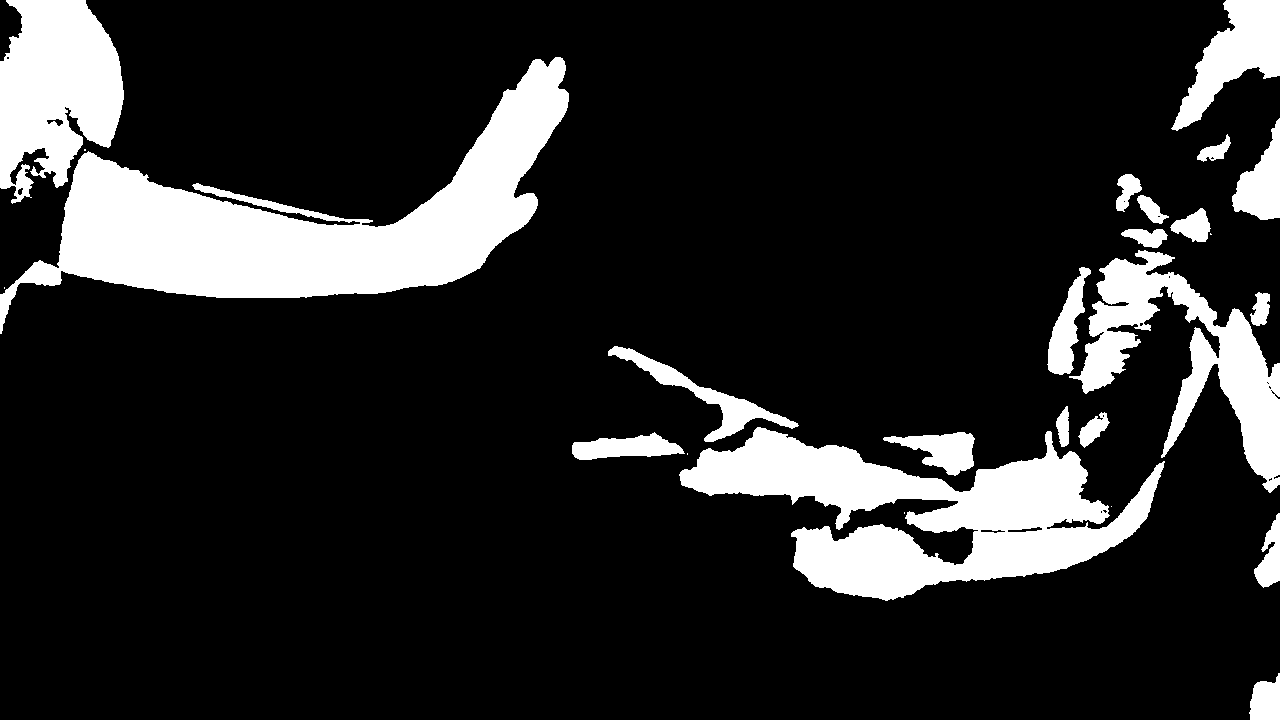
\includegraphics[width=0.28\textwidth]{\ImgPath/rys/bs/lsbp.png}}
	\caption{Przykładowe obrazy biorące udział w wyborze odpowiedniej funkcji z biblioteki OpenCV usuwającej tło}
\end{figure}

Po przeprowadzeniu licznych testów wywnioskowałem, że najlepszą metodą w mojej pracy inżynierskiej będzie funkcja z biblioteki OpenCV \textit{BackgroundSubtractorKNN}. Uważam, że na przetestowanych próbkach segmentacja ruchu metodą tą dawała najlepsze rezultaty w porównaniu z innymi przetestowanymi metodami. Parametry funkcji przyjęły następującą końcową wartość:
\begin{enumerate}
	\item history: 200
	\item dist2Threshold: 8
	\item detectShadows: false
\end{enumerate}

\begin{figure}[H]
	\centering
	\subfigure[Znak papieru]
	{\label{fig:a}\includegraphics[width=0.3\textwidth]{\ImgPath/rys/bs/papier.png}}
	\subfigure[Gest kamienia]
	{\label{fig:b}\includegraphics[width=0.3\textwidth]{\ImgPath/rys/bs/kamien.png}}
	\subfigure[Gest nożyc]
	{\label{fig:b}\includegraphics[width=0.3\textwidth]{\ImgPath/rys/bs/nozyce.png}}
	\caption{Uzyskane rezultaty metodą BackgroundSubtractorKNN z biblioteki OpenCV}
\end{figure}


Można zauważyć, że wykonywany ruch dłonią jest bardzo widoczny, jednakże dodatkowo zawarta jest duża ilość szumu. Pozbycie się elementów dodatkowych, nieinteresujących nas części obiektów przedstawię w kolejnych podrozdziałach o detekcji kolorów oraz w podrozdziale o filtracji szumu. 

\section{Detekcja kolorów}
Równolegle do segmentacji obiektów w ruchu, zająłem się detekcją obiektów o określonym kolorze. W swojej pracy inżynierskiej założyłem, że każdy wykonywany gest jest pokazywany w niebieskiej rękawiczce, w celu łatwiejszej segmentacji dłoni. Nie został użyty tradycyjny kolor skóry ze względu na fakt, że oprócz detekcji dłoni, spowodowałby także segmentację innych części ciała takich jak twarz. Wszystko to mogłoby spowodować mniej precyzyjne rozpoznawanie gestu.

Wybrałem kolor niebieski ze względu na fakt, że jest to kolor dobrze rozróżniający się od innych, na który nie wpływa aż tak znacząco moc oświetlenia.
Jako że każdy gest wykonywany jest w niebieskiej rękawiczce, mogłem wykorzystać ten fakt i przy pomocy modelu HSV określić zakres kątów barwy w tym modelu. 
 
Na modelu HSV można łatwo zaobserwować, że kolor niebieski znajduje się w pewnym przedziale składowej H modelu HSV. To pozwala na zdecydowanie łatwiejsze określenie zakresu niż w przypadku modelu RGB.  

Przedział składowej H w modelu HSV, został tak dobrany, aby zawierał większość barw zbliżonych do niebieskiej. To pozwoliło na rozszerzenie liczby wykrytych pikseli, a w efekcie lepiej wysegmentowaną dłoń. Jednakże wszystko to również niesie za sobą różnego rodzaju szumy, obiekty który również są barwy niebieskiej, jednakże które nie są związane z obiektem dłoni.
\begin{figure}[H]
	\centering
	\subfigure[Znak papieru]
	{\label{fig:a}\includegraphics[width=0.3\textwidth]{\ImgPath/rys/detekcja_koloru/papier.png}}
	\subfigure[Gest kamienia]
	{\label{fig:b}\includegraphics[width=0.3\textwidth]{\ImgPath/rys/detekcja_koloru/kamien.png}}
	\subfigure[Gest nożyc]
	{\label{fig:b}\includegraphics[width=0.3\textwidth]{\ImgPath/rys/detekcja_koloru/nozyce.png}}
	\caption{Rezultaty detekcji dłoni w niebieskiej rękawiczce}
\end{figure}

\paragraph{Zakres modelu HSV jaki wykorzystałem w swojej pracy inżynierskiej:}
\begin{enumerate}
	\item od HSV (98,50,20)
	\item do HSV (130,255,255)
\end{enumerate}
\mbox{} \\

Segmentacje niosą ze są różnego rodzaju szum, jednakże jeżeli połączymy detekcję koloru niebieskiego z detekcją ruchu, która została opisana w poprzednim podrozdziale, może pozbyć się w większości tych niechcianych elementów. 

\begin{figure}[H]
	\centering
	\subfigure[Znak papieru]
	{\label{fig:a}\includegraphics[width=0.3\textwidth]{\ImgPath/rys/bs_color/papier.png}}
	\subfigure[Gest kamienia]
	{\label{fig:b}\includegraphics[width=0.3\textwidth]{\ImgPath/rys/bs_color/kamien.png}}
	\subfigure[Gest nożyc]
	{\label{fig:b}\includegraphics[width=0.3\textwidth]{\ImgPath/rys/bs_color/nozyce.png}}
	\caption{Rezultaty detekcji dłoni w niebieskiej rękawiczce oraz wykrywania ruchu}
\end{figure}

Jak widzimy większość z niepożądanych szumów została usunięta za sprawą połączania dwóch masek binarnych. Możemy też zaobserwować, że nie wszystko zostało prawidłowo przefiltrowane, mogły też pozostać tzw. dziury binarne czyli części obiektów, które nie zostały zakwalifikowane jako części obiektu, a nimi faktyczne są. 

Wszystko to powoduje, że konieczne są kolejne filtracje szumów. W tym przypadku wykorzystałem operacje morfologiczne na obrazach binarnych, które opiszę w następnym podrozdziale.  

\section{Filtracja szumów}
Połączenie iloczynowe maski binarnej uzyskanej z segmentacji obiektów w ruchu oraz maski binarnej z obiektami o określonym kolorze niesie za sobą możliwe niedokładności, które dla polepszenia efektowności rozpoznawania gestów należy zminimalizować. Odbywa się to poprzez zastosowanie operacji morfologicznych na obrazie binarnym. 

\paragraph{Dodatkowe elementy:} \mbox{} \\
\indent
Pierwszym problemem po wygenerowaniu maski binarnej można uznać wszystkie dodatkowe elementy, które nie powinny być zakwalifikowane jako część dłoni. Segmentacja elementów obrazu w ruchu może nieść ze sobą różnego rodzaju szum spowodowany tym, że inne obiekty, różne od naszej dłoni też mogą się poruszać, co w wyniku generacji maski binarnej zostaną też wzięte pod uwagę. Kolejnym problem są także wszystkie te piksele, które są koloru niebieskiego lub też są zbliżone do niego, a więc przy wyłuskiwaniu wszystkich pikseli o kolorze rękawiczki, czyli o kolorze niebieskim, zostaną również uwzględnione jako obiekt.
 
\begin{figure}[H]
	\centering
	\subfigure[Maska binarna przed operacją erozji morfologicznej]
	{\label{fig:a}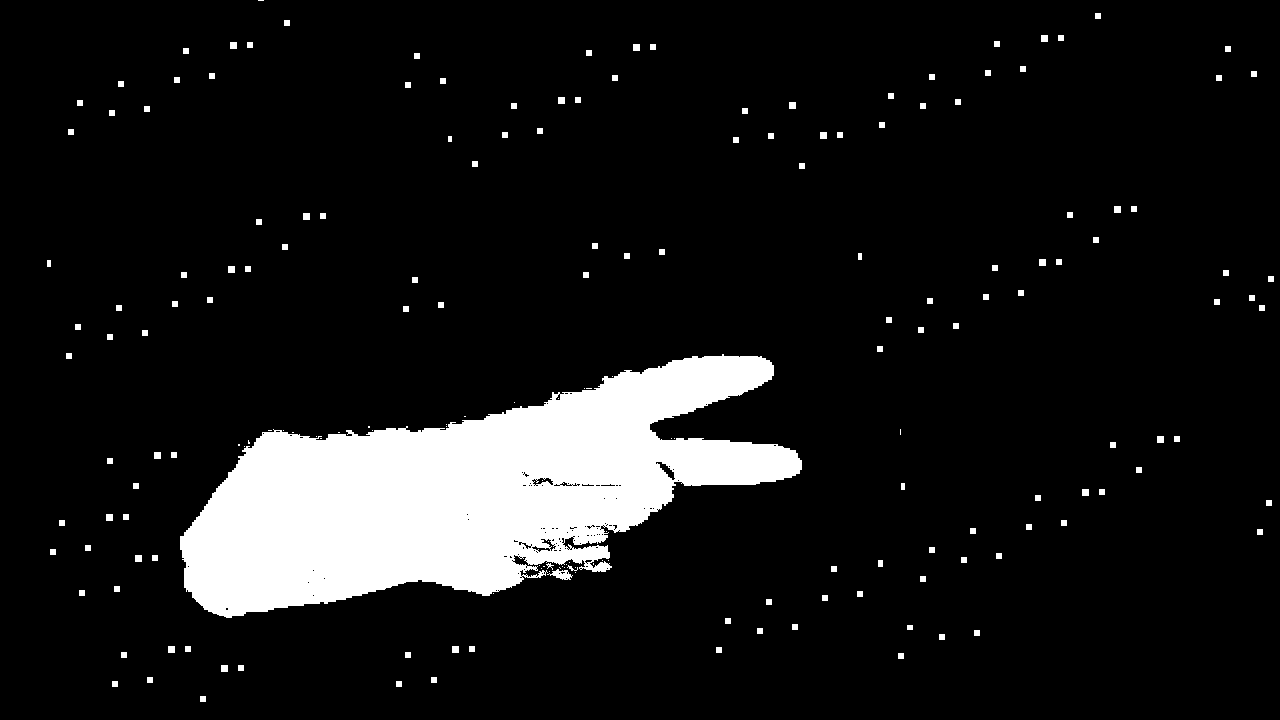
\includegraphics[width=0.45\textwidth]{\ImgPath/rys/szumy/przed_erozja.png}}
	\subfigure[Maska binarna po operacji erozji morfologicznej]
	{\label{fig:b}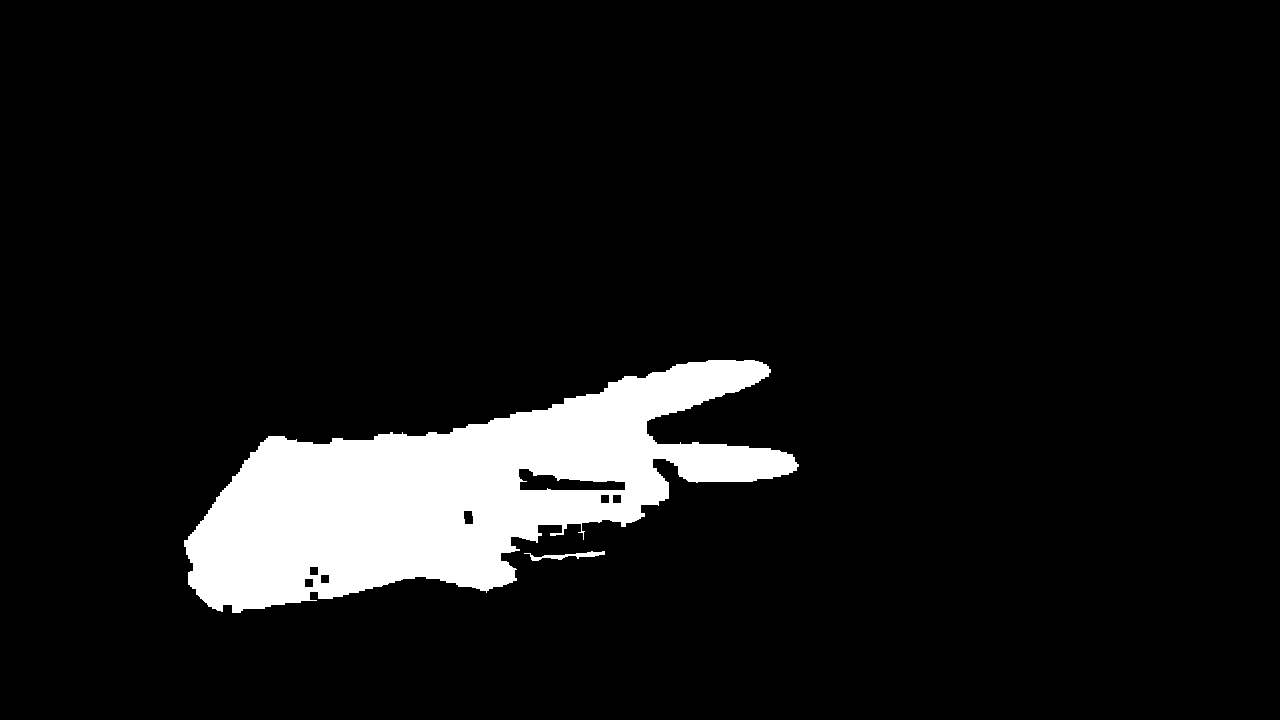
\includegraphics[width=0.45\textwidth]{\ImgPath/rys/szumy/po_erozji.png}}
	\caption{Zastosowanie operacji morfologicznej erozji z elementem strukturalnym kwadratu o boku 7 pikseli}
\end{figure}

Zastosowanie operacji morfologicznej erozji na masce binarnej powoduje usunięcie elementów niechcianych, które są traktowane jako dodatkowy, niepotrzebny szum. W swojej pracy inżynierskiej wykorzystałem w pierwszym kroku filtracji masek binarnych operację morfologiczną erozji z elementem strukturalnym kwadratem o boku 7. Wykorzystanie takiej operacji w mojej ocenie dało zadowalające efekty, które pozwolą na dokładniejsze rozpoznawanie gestów.

\paragraph{Ubytku w dłoni:} \mbox{} \\ \indent
Oprócz pozbycia się dodatkowych elementów na obrazie binarnym należy także, wypełnić luki, które mogły się pojawić podczas segmentacji obiektów w ruchu oraz przy uzyskiwaniu maski binarnej z obiektami o określonym kolorze. Są one spowodowane tym, że pewne części z obrazów podczas tych operacji nie zostały prawidło zakwalifikowane. Zbyt mocne lub też zbyt słabe światło czy też pojawiające się cienie mogły wpłynąć na kolor niebieskiej rękawiczki, a przez to spowodować niedokładne wykrycie. Również gest ręki mógł być bardzo powolny, a przez co nie zostać prawidło uznanym  przez operacje segmentacji ruchu. Jednakowo też dynamiczny ruch ręku w połączeniu z występujących w otoczeniu światłem wpływa na odbierany kolor rękawiczki. Należy też dodatkowo wziąć pod uwagę dziury w obrazie binarnym, który mogły wyniknąć z operacji morfologicznej erozji, która została zastosowana jako pierwsza. 

\begin{figure}[H]
	\centering
	\subfigure[Maska binarna przed operacją morfologiczną dylatacji]
	{\label{fig:a}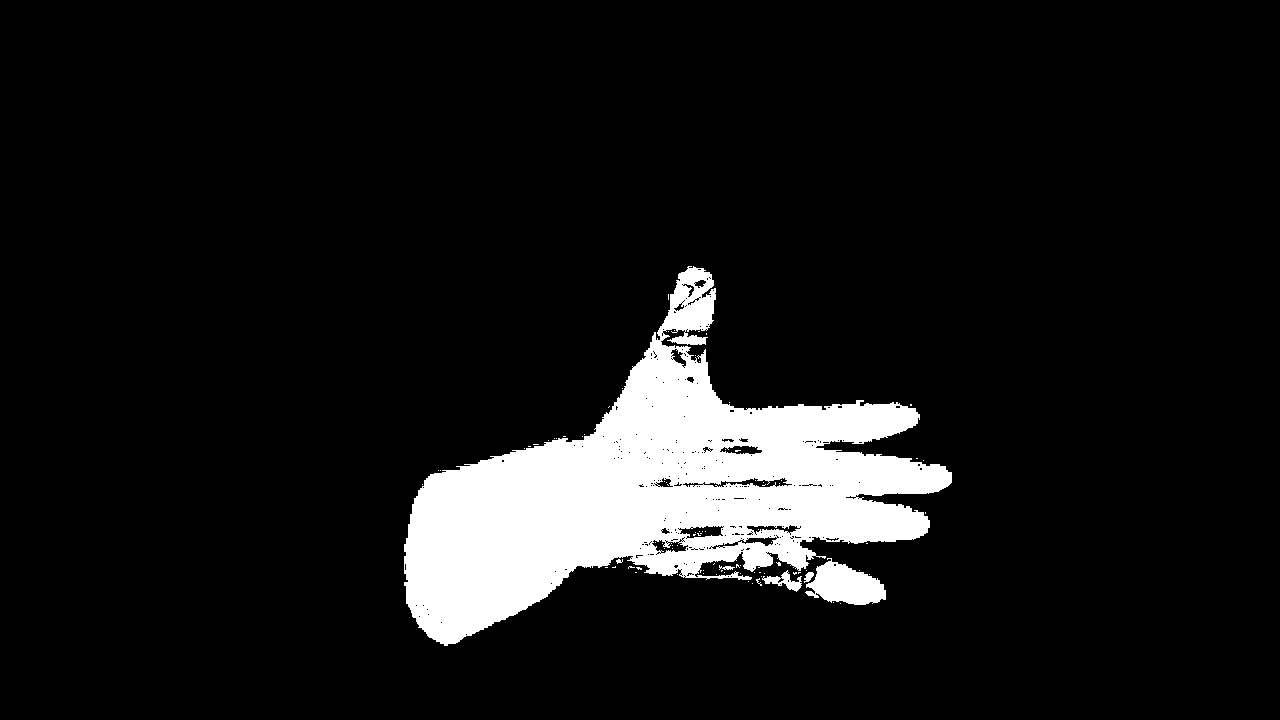
\includegraphics[width=0.45\textwidth]{\ImgPath/rys/szumy/przed_dylatacja.png}}
	\subfigure[Maska binarna po operacji morfologicznej dylatacji]
	{\label{fig:b}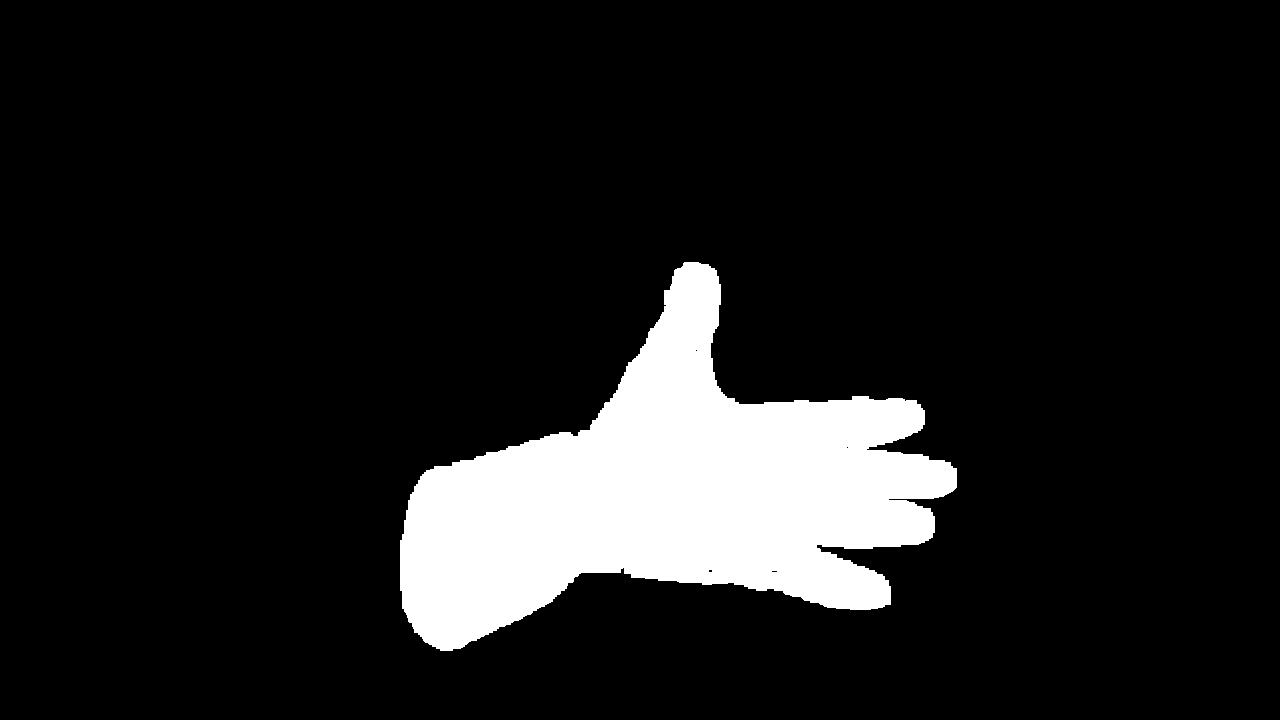
\includegraphics[width=0.45\textwidth]{\ImgPath/rys/szumy/po_dylatacji.png}}
	\caption{Zastosowanie operacji morfologicznej dylatacji z elementem strukturalnym kwadratu o boku 21 pikseli}
\end{figure}

Zastosowanie operacji morfologicznej dylatacji na masce binarnej powoduje wypełnienie dziur, które mogły wystąpić w masce binarnej. W swojej pracy inżynierskiej do pozbycia się różnego rodzaju dziur w maskach binarnych użyłem operacji morfologicznej dylatacji z elementem strukturalnym kwadratu o boku 21. 

\begin{figure}[H]
	\centering
	\subfigure[Gest kamienia przed filtracją ]
	{\label{fig:a}\includegraphics[width=0.45\textwidth]{\ImgPath/rys/szumy/1.png}}
	\subfigure[Gest kamienia po filtracji]
	{\label{fig:b}\includegraphics[width=0.45\textwidth]{\ImgPath/rys/szumy/2.png}}
	\caption{Przykładowe maski binarne po zastosowaniu operacji morfologicznych erozji oraz dylatacji z elementami strukturalnymi kwadratu o boku 7 dla erozji oraz kwadratu o boku 21 dla operacji dylatacji}
\end{figure}

W swojej pracy inżynierskiej zastosowałem następujące operacje do przefiltrowania masek binarnych: 
\begin{enumerate}
	\item Operację morfologiczną erozji na masce binarnej z elementem strukturalnym kwadratu o boku 7
	\item Operację morfologiczną zamknięcia z elementem strukturalnym kwadratu o boku 9 na wyjściowej masce binarnej uzyskanej w podpunkcie nr 1
	\item Operację morfologiczną dylatacji z elementem strukturalnym kwadratu o boku 21 na wyjściowej masce binarnej uzyskanej w podpunkcie nr 2
\end{enumerate}

\begin{figure}[H]
	\centering
	\subfigure[Gest papieru ]
	{\label{fig:a}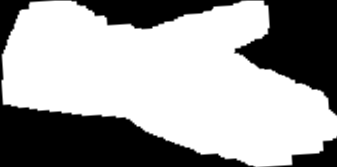
\includegraphics[width=0.3\textwidth]{\ImgPath/rys/szumy/p.png}}
	\subfigure[Gest kamienia]
	{\label{fig:b}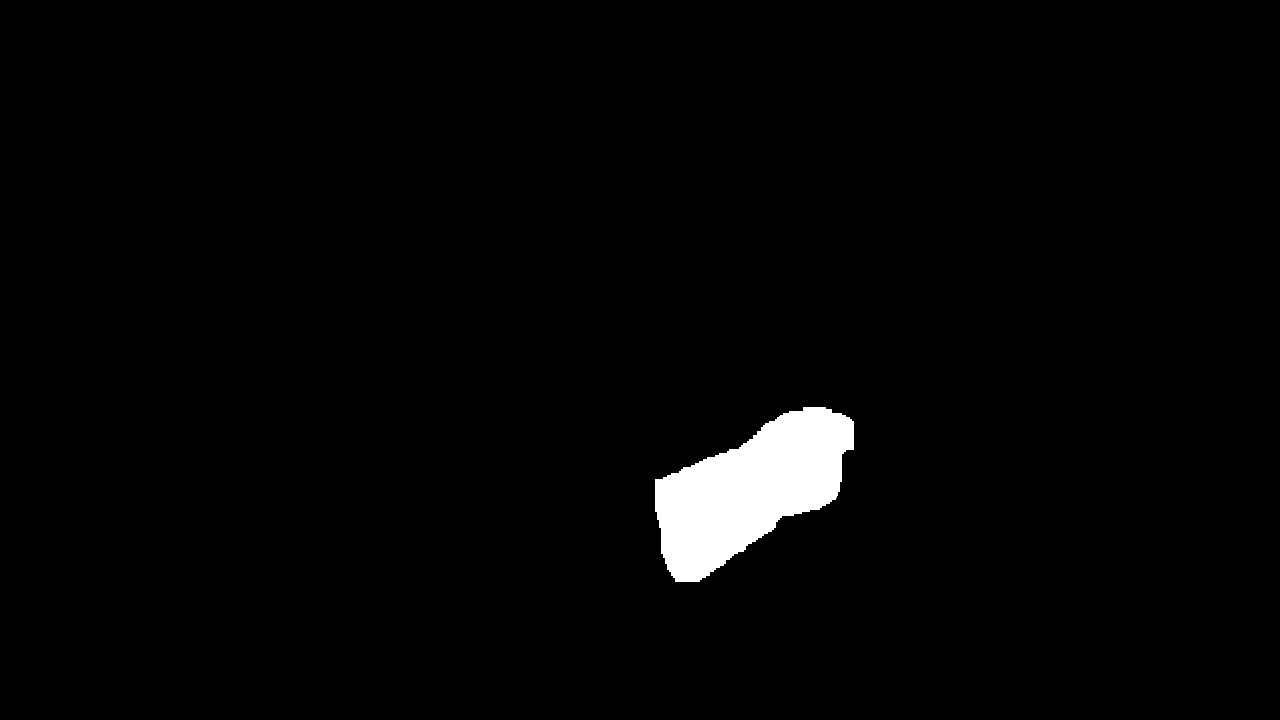
\includegraphics[width=0.3\textwidth]{\ImgPath/rys/szumy/k.png}}
	\subfigure[Gest nożyc]
	{\label{fig:b}\includegraphics[width=0.3\textwidth]{\ImgPath/rys/szumy/n.png}}
	\caption{Przykłady efektów wykonanej filtracji, która została powyżej opisana}
\end{figure}

Cała filtracja  w mojej ocenie dała bardzo dobre rezultaty, które znacząco polepszyły prawidłową segmentację dłoni, a przez to w późniejszych krokach dokładniejsze rozpoznawanie dłoni.

\section{Znajdowanie obiektów}
Ostatnim etapem przetwarzania obrazów w mojej pracy inżynierskiej było wydzielenie z maski binarnej prostokąta, zawierającego w sobie całą wysegmentową wcześniej dłoń, bez ogólnego tła. Dzięki czemu jesteśmy wstanie analizować jedynie tę część maski binarnej, która zawiera w sobie całą dłoń, bez zbędnych innych elementów.

Znajdowanie to polegało na wyszukaniu prostokąta na całej masce binarnej, która będzie miała największe pole ze wszystkich znalezionych konturów na obiektach z maski binarnej. 

\begin{figure}[H]
	\centering
	{\label{fig:a}\includegraphics[width=0.60\textwidth]{\ImgPath/rys/obcinanie/znalezienie.jpg}}
	\caption{Zaznaczenie na czerwono prostokąta o największym polu, który zawiera w sobie całościowo obiekt}
\end{figure}

Po znalezieniu takiego prostokąta następowało przycięcie maski binarnej do odpowiednich rozmiarów zgodnie ze znalezionym prostokątem o największym polu. Prostokąt ten jest przyległy przez obiekt binarny z każdej swojej strony, co oznacza, że większe przycięcie nie jest możliwe, bez zmniejszania znalezionego obiektu.

\begin{figure}[H]
	\centering
	{\label{fig:b}\includegraphics[width=0.50\textwidth]{\ImgPath/rys/obcinanie/obcinanie.png}}
	\caption{Obcięcie zgodnie ze znalezionym prostokątem}
\end{figure}
\paragraph{Etapy przycięcia maski binarnej:}
\begin{enumerate}
	\item Przypisz do obecnie znalezionego największego pola prostokąta wartość~0
	\item Znajdź wszystkie kontury obiektów na masce binarnej
	\item Dla każdego konturu wykonaj:
	\begin{enumerate}
		\item Oblicz współrzędne lewego górnego oraz prawego dolnego wierzchołka prostokąta, który będzie otaczał analizowany kontur 
		\item Oblicz pole powierzchni tak utworzonego prostokąta
		\item Jeżeli pole powierzchni utworzonego prostokąta jest większe niż pole powierzchni obecnie znalezionego największego prostokąta, to traktur tą powierzchnię jako największą i dodatkowo zapamiętaj współrzędne prostokąta
	\end{enumerate}
	\item Przytnij maskę binarną o zapamiętanych wierzchołkach największego znalezionego prostokąta
\end{enumerate}

Efekt końcowy wysegmentowania dłoni zawiera w sobie obiekt binarny reprezentujący dłoń, którą jest wykonywany gest. Zostanie on wykorzystany przez klasyfikatory opisane w następnych podrozdziałach.

\begin{figure}[H]
	\centering
	\subfigure[Gest papieru ]
	{\label{fig:a}\includegraphics[width=0.3\textwidth]{\ImgPath/rys/obcinanie/p.png}}
	\subfigure[Gest kamienia]
	{\label{fig:b}\includegraphics[width=0.3\textwidth]{\ImgPath/rys/obcinanie/k.png}}
	\subfigure[Gest nożyc]
	{\label{fig:b}\includegraphics[width=0.3\textwidth]{\ImgPath/rys/obcinanie/s.png}}
	\caption{Końcowa segmentacja dłoni}
\end{figure} 

\section{Dobór i ocena cech}
Po wysegmentowaniu gestów dla uczenia maszynowego przeszedłem do etapu opisu odpowiednimi cechami zgromadzonego materiału. Skupiłem się, na właściwościach binarnych jakie one przedstawiają.

\paragraph{Zdecydowałem się, że gesty będę opisywał za pomocą następujących cech:}
\begin{itemize}
	\item Stosunek szerokości do długości rozmiarów maski binarnej
	\item Stosunek powierzchni znalezionego obiektu dłoni do powierzchni całego obrazu
	\item Stosunek powierzchni otoczki wypukłej utworzonej na znalezionej dłoni do powierzchni całego obrazu
\end{itemize}

Pierwszym krokiem przy analizowaniu cech opisujących dane było wyliczenie średnich w obrębie określonego gestu.

\begin{table}[H]
	\centering
	\begin{tabularx}{\textwidth}{|X|l|l|l|}
		\hline
		\textbf{Nazwa cechy} & \textbf{Papier} & \textbf{Kamień} & \textbf{Nożyce} \\ 
		
		\hline
		Stosunek szerokości do długości & 0.43 & 0.59 & 0.78 \\ 
		
		\hline
		Stosunek powierzchni obiektu dłoni do powierzchni całego obrazu & 0.48 & 0.38 & 0.84 \\ 
		
		\hline
		Stosunek powierzchni otoczki wypukłej utworzonej na znalezionej dłoni do powierzchni całego obraz & 0.35 & 0.62 & 0.84 \\ 
		\hline
	\end{tabularx}

	\caption{Wartości średnie}
\end{table}

Przy ocenie jakości dobranych cech wykorzystałem odchylenie standardowe. Dzięki niemu byłem wstanie porównać jak dana cecha jest porozrzucana w obrębie określonego gestu.

\begin{table}[H]
	\centering
	\begin{tabularx}{\textwidth}{|X|l|l|l|}
		\hline
		\textbf{Nazwa cechy} & \textbf{Papier} & \textbf{Kamień} & \textbf{Nożyce} \\ 
		
		\hline
		Stosunek szerokości do długości & 0.10 & 0.18 & 0.05 \\ 
		
		\hline
		Stosunek powierzchni obiektu dłoni do powierzchni całego obrazu & 0.09 & 0.10 & 0.04 \\ 
		
		\hline
		Stosunek powierzchni otoczki wypukłej utworzonej na znalezionej dłoni do powierzchni całego obraz & 0.10 & 0.16 & 0.05 \\ 
		\hline
	\end{tabularx}
	
	\caption{Odchylenie standardowe}
\end{table}
Odchylenie standardowe dla danej cechy, w obrębia określonego gestu nie były dużą wartością, co oznacza, że cecha ta nadaje się dobrze, aby ją wykorzystać przy rozpoznawaniu gestów.

Po przeanalizowaniu odchyleń standardowych doszedłem do wniosku, że wszystkie trzy, wcześniej wybrane cechy są odpowiednie, aby je wykorzystać do stworzenia klasyfikatora.  

\section{Rozpoznawanie gestów przy pomocy klasyfikatora KNN}
Dla klasyfikatora KNN przygotowałem zestaw cechy opisujących maskę binarną z poprzedniego podrozdziału.

Każda z cech została poddana etapowi normalizacji w postaci standaryzacji. Została ona przeprowadzona zgodnie ze wzorem: $ Z = \dfrac{x - \mu}{\sigma} $, gdzie x - wartość przed normalizacją, $\mu$ - średnia, $\sigma$ - odchylenie standardowe

Klasyfikator został oparty na klasycznej odległości euklidesowej. Zbiór danych, który został opisany w poprzednich podrozdziałach składał się z 1050 różnych próbek danych. Został on podzielony w stosunku 8:2, dzięki czemu zbiór uczący liczył 855 próbek, zaś zbiór weryfikacyjny zawierał 195 próbek. 


\begin{table}[H]
	\centering
	\begin{tabularx}{\textwidth}{|X|X|X|X|}
		\hline
		\textbf{Wartość parametru k} & \textbf{Średnia dokładność klasyfikatora}    \\ 
		
		\hline
		3 & 83.76\% \\ 
		\hline
		\textbf{5} & \textbf{86.08}\% \\
		\hline
		7 & 82.41\% \\
		\hline
		9 & 81.68\% \\
		\hline
	\end{tabularx}
	
	\caption{Skuteczność KNN w zależności od parametru k}
\end{table}
	
Z wykonanych analiz dokładności klasyfikatora KNN w zależności od parametru k wynika, że najlepsze efekty można było osiągnąć używając go z parametrem k o wartości 5, który działał ze średnią dokładnością 86.08\%.
\section{Rozpoznawanie gestów przy pomocy sieci neuronowej}
\subsection{Sieć neuronowa oparta o cechy}
	Analogicznie jak w przypadku klasyfikatora KNN również i  kolejny klasyfikator oparłem na wyznaczonych wcześniej cechach.
	
	Sieć została stworzona w języku Python, korzystając z biblioteki TensorFlow oraz jako wysokopoziomowe API sieci neuronowych wykorzystałem bibliotekę Keras.
	
	\paragraph{Sieci neuronowe, które wykorzystywałem przy budowie klasyfikatora składały się z następujących części:}
	\begin{enumerate}
		\item Warstwa wejściowa
		\item Jedna warstwa ukryta
		\item Warstwa wyjściowa
	\end{enumerate}

	\noindent
	Każda z cech została poddana etapowi normalizacji w postaci standaryzacji, która zdecydowanie korzystnie wpływała na skuteczność klasyfikacji.
	
	Zbiór uczący sieci neuronowe zawierał 855 próbek, zaś zbiór weryfikacyjny zawierał w sobie 195 próbek. Każdy z trzech gestów miał po 350 próbek, zaś przydział do odpowiedniego zbioru odbywał się w sposób losowy.
	
	Warstwa wyjściowa każdej z przetestowanych sieci, składała się z funkcji aktywacji softmax, której wyjście traktowałem jako prawdopodobieństwo danego z trzech gestów. Każdy z trzech neuronów wyjściowych oznaczył właśnie to prawdopodobieństwo w następującej kolejności:
	\begin{enumerate}
		\item gest papieru
		\item gest kamienia
		\item gest nożyc
	\end{enumerate}
	\mbox{}\\
	\begin{table}[H]
		\centering
		\begin{tabularx}{\textwidth}{|X|X|X|X|}
			\hline
			\textbf{} & \textbf{ReLU funkcją aktywacji} & \textbf{Sigmoid funkcją aktywacji}  & \textbf{Tanh funkcją aktywacji}  \\ 
			
			\hline
			2 neurony w warstwie ukrytej & 57.54\% & 63.29\% & 74.28\% \\ 
			
			\hline
			4 neurony w warstwie ukrytej & 80.05\% & 64.52\% & 81.35\% \\
			
			\hline
			6 neuronów w warstwie ukrytej & \textbf{83.43}\% & \textbf{69.01}\% & \textbf{83.08}\% \\
			
			\hline
			8 neuronów w warstwie ukrytej & 81.59\% & 67.54\% & 77.26\% \\
			
			\hline
			10 neuronów w warstwie ukrytej & 80.03\% & 64.21\% & 78.11\% \\
			
			\hline
			12 neuronów w warstwie ukrytej & 79.89\% & 57.63\% & 76.41\% \\
			
			\hline
			15 neuronów w warstwie ukrytej & 81.28\% & 65.59\% & 79.62\% \\
			
			\hline
			20 neuronów w warstwie ukrytej & 78.82\% & 61.77\% & 80.09\% \\
			
			\hline
			25 neuronów w warstwie ukrytej & 78.55\% & 54.23\% & 77.78\% \\
			
			\hline
			50 neuronów w warstwie ukrytej & 77.73\% & 60.19\% & 79.13\% \\ 
			\hline
		\end{tabularx}
		
		\caption{Skuteczność sieci neuronowej}
	\end{table}
   	Pierwszym zbiorem sieci jaki przetestowałem były to sieci z jedną warstwą ukrytą. Do uczenia sieci wykorzystywałem metodę \textit{GradientDescentOptimizer} z parametrem uczenia równym 0.01. Zaś sama sieć została uruchomiana dla 100 epok uczących. Ilość neuronów w warstwie ukrytej oraz funkcje aktywacji dla tej warstwy i warstwy wejściowej były to parametry, które doświadczalnie zmieniałem.

	
	Po przeprowadzonych doświadczeniach okazało się, że najlepsze wyniki można było uzyskać siecią neuronową składającą się z 6 neuronów w warstwie ukrytej, przy wykorzystywaniu funkcji aktywacji ReLU w warstwie wejściowej oraz w warstwie ukrytej. 
	
	Można również zauważyć, że sieć niezależnie od funkcji aktywacyjnej dla 6 neuronów w warstwie ukrytej zawsze dawała najlepsze rozwiązanie.
	
	W następnym etapie swojej pracy przeanalizowałem, wpływ ilości epok uczących. Testowanie odbyło się na sieci, która dała najlepsze rezultaty w poprzednim doświadczeniu.

	\begin{figure}[H]
		\centering
		{\label{fig:b}\includegraphics[width=0.90\textwidth]{\ImgPath/rys/opoki.png}}
		\caption{Skuteczność uczenia sieci w zależności od ilości epok uczenia}
	\end{figure}

	Na wykresie można zaobserwować bardzo dynamiczny wzrost skuteczności uczenia, dla pierwszych 50 epok. Kolejnym 50 epokach następuje również sporo wzrost skuteczności, jednakże już nie tak gwałtowny. Uczenie przy ponad 100 opokach daje to coraz mniejszy wzrost skuteczności uczenia, co można z łatwością zobaczyć na wykresie. Analiza ta spowodowała, że sieci neuronowe poddawałem uczeniu dla 100 epok.
	
	Ostatnią własność, którą przeanalizowałem był dobór parametru szybkości uczenia w metodzie \textit{GradientDescentOptimizer}.
	
	\begin{table}[H]
		\centering
		\begin{tabularx}{\textwidth}{|X|X|X|X|}
			\hline
			\textbf{Szybkość uczenia} & \textbf{Skuteczność sieci neuronowej}    \\ 
			
			\hline
			0.001 & 67.19\% \\ 
			
			\hline
			0.010 & \textbf{83.43}\% \\
			
			\hline
			0.020 & 78.91\% \\
			
			\hline
			0.050 & 80.37\% \\
			
			\hline
			0.100 & 80.34\% \\
			
			\hline
			0.150 & 79.88\% \\
			
			\hline
			0.200 & 80.02\% \\
			
			\hline
			0.250 & 81.11\% \\
			
			\hline
			0.500 & 82.78\% \\
			\hline
		\end{tabularx}
		
		\caption{Skuteczność sieci neuronowej w zależności od współczynnika szybkości uczenia}
	\end{table}

	Większość z prób była do siebie zbliżona skutecznością. W wykonanych doświadczeniach sieć dawała najlepsze rozwiązania dla parametru szybkości uczenia o wartości: 0.01.
	

	\paragraph{Przeprowadzona analiza pozwoliła ustalić ostateczne parametry sieci:}
	\begin{itemize}
		\item Sieć składa się z następujących warstw: warstwa wejściowa, jedna warstwa ukryta, warstwa wyjściowa
		\item Warstwa wejściowa składa się z trzech neuronów reprezentujące wartości cech dla danej próbki, zaś funkcją aktywacji neuronów tej warwie jest funkcja ReLU
		\item Warstwa ukryta składa się z 6 neuronów, a funkcja aktywacji każdego z nich to również ReLU
		\item Warstwa wyjściowa składa się z trzech neuronów, które reprezentują prawdopodobieństwo gestu w kolejności: papier, kamień, nożyce. Funkcja aktywacja dla każdego z neuronów to softmax.
		\item Sieć była uczona na 100 epokach
		\item Jako metodę uczenia uczenia wykorzystałem dostępny w bibliotece Keras GradientDescentOptimizer, ze współczynnikiem uczenia 0.01
		\item Sieć była uczona 855 próbkami zbioru uczącego
		\item Sieć była testowana 195 próbkami zbioru weryfikującego
	\end{itemize}
	\mbox{}
	\\
	Sieć z podanymi wyżej parametrami dała średnią skuteczność na poziomie 83.43\%. Jest to wartość zadowalająca, zbliżona do wartości jaka została uzyskana za pomocą klasyfikatora KNN.
\subsection{Sieć neuronowa oparta o wartości pikseli obrazu binarnego}


	Kolejnym podejściem do klasyfikacji była analiza wysegmentowanej dłoni gestu siecią neuronową tym razem bez opisywania gestu cechami, lecz użyciem całego otrzymanego wcześniej obrazu binarnego.
	
	Po procesie segmentacji dłoni z gestem, opisanym w poprzednich podrozdziałach, należało ustandaryzować rozmiar wcześniej otrzymanego obrazu binarnego, który został wykorzystany jako element wejścia dla sieci neuronowej. Ustaliłem, że rozmiar będzie wynosił 60 pikseli szerokości oraz 25 pikseli wysokości. Stosunek obu wartości chciałem tak dobrać, aby zachował jak najbardziej ogólną jego wartość dla wszystkich obrazów binarnych z wykorzystywanego zbioru danych. Zmniejszenie rozmiaru, ma również korzystny wpływ na szybkość działania sieci, jednakże w wyniku czego tracimy pewne dostępne szczegóły na obrazie. Poza zmianą wymiarów zbiór danych był analogiczny do wykorzystywanych poprzednio.

	Sieć została stworzona w języku Python, korzystając z biblioteki TensorFlow oraz jako wysokopoziomowe API sieci neuronowych wykorzystałem bibliotekę Keras.

	
	\paragraph{Sieci neuronowe, które wykorzystywałem przy budowie klasyfikatora składały się z następujących części:}
	\begin{enumerate}
		\item Warstwa wejściowa
		\item Jedna warstwa ukryta
		\item Warstwa wyjściowa
	\end{enumerate}
	
	Jako elementy wejścia były wykorzystywane wysegmentowane wcześniej obrazy dłoni z gestem i skonwertowane do rozmiaru 60 pikseli szerokości i 25 pikseli wysokości. 
	
	Zmniejszenie obrazu binarnego niosło za sobą również zmianę kodowanie obrazu. Po wykonaniu tej operacji cały zbiór danych był kodowany jako zbiór obrazów szarościowych.
		
	Do warstwy wejściowej sieci, podane zostały wartości pikseli obrazów szarościowych o rozmiarze 25x60. 
	
	Ilość neuronów w warstwie ukrytej był to parametr, który doświadczalnie zmieniałem. Funkcja aktywacji jaką wykorzystałem dla tej warstwy była to funkcja RuLU.

	Warstwa wyjściowa każdej z przetestowanych sieci, składała się z funkcji aktywacji softmax, której wyjście traktowałem jako prawdopodobieństwo danego z trzech gestów. Każdy z trzech neuronów warstwy wyjścia oznaczał właśnie to prawdopodobieństwo w następującej kolejności:
	\begin{enumerate}
		\item gest papieru
		\item gest kamienia
		\item gest nożyc
	\end{enumerate}

	\paragraph{Budowa sieci neuronowej korzystając z biblioteki Keras:}
	\begin{lstlisting}[language=Python]
   model = keras.Sequential([
     keras.layers.Flatten(input_shape=(25, 60)),
     keras.layers.Dense(256, activation=tf.nn.relu),
     keras.layers.Dense(3, activation=tf.nn.softmax)
   ])
	\end{lstlisting}
	
	Do uczenia sieci neuronowych wykorzystywałem metodę dostępną w bibliotece Keras GradientDescentOptimizer z parametrem uczenia równym 0.01. Zaś sama sieć została uruchomiana dla 100 epok. 
	
	\paragraph{Zanotowałem następujące dokładności rozpoznawania siecią przy wyżej wymienionych parametrach:}
	
	\mbox{}\\
	
	\begin{table}[H]
		\centering
		\begin{tabularx}{\textwidth}{|X|X|X|X|}
			\hline
			\textbf{Liczba neuronów w warstwie ukrytej sieci} & \textbf{Dokładność klasyfikacji} \\ 
			
			\hline
			32  & 98.13\% \\ 
			
			\hline
			64  & 98.46\% \\
			
			\hline
			128  & 99.18\% \\
			
			\hline
			256  & \textbf{99.58}\% \\
			
			\hline
			512  & 98.88\% \\
			
			\hline
		\end{tabularx}
		
		\caption{Skuteczność sieci neuronowej}
	\end{table}

	Powyższe wartości dokładności rozpoznawania gestów przez sieć neuronową pokazują, że wyśmienicie sobie radzi z klasyfikacją gestów. Najlepsze rezultaty dawała sieć zbudowana z 256 neuronów w warstwie ukrytej. Średnia jej skuteczność to ponad 99\% co sprawia, że rozpoznawanie gestów można uznać praktycznie za bezbłędne. 	

\chapter{Podsumowanie}
	W niniejszej pracy inżynierskiej opisałem podejście do rozpoznawania gestów na przykładzie gry papier, kamień, nożyce. 
	
	Proces segmentacji dłoni składał się z wielu pomniejszych etapów. Pierwszym z nich była akwizycja zbioru danych. Proces ten był pracochłonny, ponieważ należało zebrać materiał od kilku różnych osób i opowiedzieć im o ich stosunkowo klarownym zadaniu jakim było pokazywanie gestów. 
	
	Zbieranie danych było etapem dosyć prostym, jednakże analiza zgromadzonego materiału wymagała dużej ilości włożonej pracy.
	
	Kolejnym etapem mojej pracy była detekcja obiektów w ruchu oraz o kolorze niebieskim. Uważam osobiście, że był to jeden z najtrudniejszych etapów w mojej pracy. Segmentacja niosła za sobą dużą ilość szumu, którego należało odpowiednio przefiltrować. Był to proces dla mnie bardzo żmudny, ponieważ do klasycznych metod opisanych w tej pracy należało dobrać odpowiednie parametry i ich kolejność wykonywania. Były to wielogodzinne prace służące, aby uzyskać jak najlepszy efekt. Wielokrotnie zdarzało się, że parametry dobrane dla jednego zestawu danych w drugim całkowicie psuły efekt wcześniejszej detekcji. To wszystko spowodowało, że należało włożyć dużo ciężkiej pracy, aby uzyskać zadowalający efekt dla całego zestawu danych.
	
	Po wykonanej pracy uważam, że trud włożony przy etapie segmentacji w dużym stopniu przyczynił się do zadowalających rezultatów w późniejszej klasyfikacji.
	
	Pierwszym podejściem do klasyfikacji dłoni był klasyfikator KNN. W pierwszym kroku należało opisać cechami zgromadzony zbiór danych. Po analizie wyselekcjonowałem trzy cechy opisujące właściwości binarne uzyskanych obrazów binarnych w procesie segmentacji. Można było zaobserwować, że każda wybrana cecha zwiększała skuteczność klasyfikacji. 
	
	Wartość parametru k dla klasyfikator KNN, była doświadczalnie ustalana. Najlepsze wyniki klasyfikacji uzyskałem dla parametru k równym 5, gdzie skuteczność wynosiła 86.08\%. Zwiększanie lub zmniejszanie tej wartości powodowało mniej dokładne wyniki.
	
	Drugim podejściem do klasyfikacji był klasyfikator oparty o sieci neuronowe, który również korzysta z tych samych cech co klasyfikator KNN. 
	
	Przy analizowaniu trzech różnych funkcji aktywacji dla warty wejściowej oraz warstwy ukrytej można było jasno zauważyć, że najgorzej spisywała się funkcja Sigmoid. Wyniki jej były zdecydowanie gorsze od pozostałych. 
	
	Rezultaty zastosowania funkcji aktywacji ReLU oraz Tanh były do siebie zbliżone, jednakże minimalnie lepiej zachowywała się funkcja ReLU, dzięki której można było uzyskać najlepsze wyniki  na poziomie 83.43\%. 
	
	Bardzo ciekawą obserwacją, było zauważenie, że sieć działała najlepiej przy 6 neuronach w warstwie ukrytej, niezależnie od używanej funkcji aktywacji.
	
	Zwiększenie ilości epok uczących zwiększała skuteczność działania sieci. Jednakże wzrost ilości epok uczących powodował większą ilość czasu potrzebnego na wykonanie koniecznych obliczeń. Uczenie powyżej 100 epok w mojej obserwacji dawało już zbyt mały zysk w stosunku do nakładów czasowych. Wszystko to spowodowało ustalenie ilości epok uczących na wartość 100.

	Ostatnim wykorzystanym klasyfikatorem był klasyfikator również oparty o sieci neuronowe, jednakże tym razem jako element wejścia był podawany cały obraz wysegmentowanej dłoni, bez opisujących go cech. Tak stworzony klasyfikator zdecydowanie przewyższył klasyfikatory wykorzystujące wcześniej dobrane cechy. Rozpoznawanie takie było praktycznie bezbłędne na zgromadzonym zestawie danych. Klasyfikator przy wykorzystaniu uzyskanych najlepszych parametrów osiągał skuteczność powyżej 99\%, co w moim przeświadczeniu jest wyśmienitym rezultatem, biorąc pod uwagę cały proces segmentacji dłoni.
	 
	W mojej ocenie słabsza skuteczność klasyfikatorów wykorzystujących opisujące cechy obrazów była spowodowana zbyt małą ich ilością. Zwiększenie ich liczby spowodowałaby obszerniejsze informacje o wysegmentowanym geście, co przyczyniłoby się do lepszej klasyfikacji. 
	
	Uważam, że cel jaki na początku swojej  pracy założyłem, czyli prawidłowe rozpoznawanie trzech gestów papieru, kamienia oraz nożyc, został osiągnięty z sukcesem. Klasyfikator oparty o sieci neuronowe pokazał jak wielkie możliwości daje wykorzystanie sztucznych sieci neuronowych, które coraz częściej są wykorzystywane w naszym codziennym życiu.

\appendix
\begin{thebibliography}{99}
\bibitem{Collins}{Andy Collins, ,,Mowa ciała'', 2002}
\bibitem{Kostkiewicz}{Paweł Kostkiewicz, Michał Syfert, ,,Interakcja człowiek-komputer'', 2010}	
\bibitem{Kinect}{Kinect SDK – Wprowadzenie, https://msdn.microsoft.com/pl-pl/\\library/kinect-sdk--wprowadzenie.aspx, dostęp: styczeń 2019}	
\bibitem{Fisher}{Len Fisher, ,,Rock, Paper, Scissors: Game Theory in Everyday Life'', 2008}	
\bibitem{Iwanowski}{Marcin Iwanowski, ,,Metody morfologiczne w przetwarzaniu obrazów cyfrowych'', 2009}
\bibitem{Malina}{Witold Malina, Maciej Smiatacz, ,,Cyfrowe przetwarzanie obrazów'', 2008}
\bibitem{opencvs2}{Background Subtraction, https://docs.opencv.org/3.4/db/d5c/\\tutorial\_py\_bg\_subtraction.html, dostęp: styczeń 2019}
\bibitem{KNN}{BackgroundSubtractorKNN, https://docs.opencv.org/3.4.1/db/d88/\\classcv\_1\_1BackgroundSubtractorKNN.html, dostęp: styczeń 2019}
\bibitem{Jankowski}{Jankowski Michał, ,,Elementy Grafiki Komputerowej'', 2006}
\bibitem{rgbhsv}{RGB to HSV color conversion, https://www.rapidtables.com/convert/\\color/rgb-to-hsv.html, dostęp: styczeń 2019}
\bibitem{Malina2}{Witold Malina, Maciej Smiatacz, ,,Rozpoznawanie obrazów'', 2010}
\bibitem{knn2}{Metoda K Najbliższych Sąsiadów, http://home.agh.edu.pl/\%7ehorzyk/\\lectures/miw/KNN.pdf, dostęp: styczeń 2019}
\bibitem{Osowski}{Osowski Stanisław, ,,Metody i narzędzia eksploracji danych'', 2013}
\bibitem{opencv}{Introduction to OpenCV-Python Tutorials, https://docs.opencv.org/\\3.4.1/d0/de3/tutorial\_py\_intro.html, dostęp: styczeń 2019}
\bibitem{opencv2}{Gloria Bueno García, Oscar Deniz Suarez, José Luis Espinosa Aranda, Jesus Salido Tercero, Ismael Serrano Gracia, Noelia Vállez Enano, ,,Learning Image Processing with OpenCV'', 2015}
\bibitem{python1}{General Python FAQ, https://docs.python.org/2/faq/general.html, dostęp: styczeń 2019}
\bibitem{python}{O'Reilly Media, ,,Learning Python 4th Edition'', 2009}
\bibitem{tiobe}{TIOBE Index for January 2019, https://www.tiobe.com/tiobe-index/, dostęp: styczeń 2019}
\bibitem{tensorflow}{TensorFlow: Large-Scale Machine Learning on Heterogeneous\\ Distributed Systems https://static.googleusercontent.com/media/\\research.google.com/en//pubs/archive/45166.pdf, dostęp: styczeń 2019}
\bibitem{tensorflowlite}{Introduction to TensorFlow Lite, https://www.tensorflow.org/lite/overview, dostęp: styczeń 2019}
\bibitem{tensorflowG}{Graphs and Sessions, https://www.tensorflow.org/guide/graphs, dostęp: styczeń 2019}
\bibitem{keras}{Introducing Keras 2, https://blog.keras.io/introducing-keras-2.html, dostęp: styczeń 2019}



\bibitem{opencvc}{Contour Properties, https://docs.opencv.org/3.4/d1/d32/tutorial\\\_py\_contour\_properties.html, dostęp: styczeń 2019}
\bibitem{convex}{Convex Hull using OpenCV in Python and C++,\\ https://www.learnopencv.com/convex-hull-using-opencv-in-python-\\and-c/, dostęp: styczeń 2019}
\bibitem{pyimagesearch}{Measuring size of objects in an image with OpenCV,\\ https://www.pyimagesearch.com/2016/03/28/measuring-size-of-\\objects-in-an-image-with-opencv/, dostęp: styczeń 2019}
\bibitem{opencvm}{Morphological Transformations, https://docs.opencv.org/3.0-beta/\\doc/py\_tutorials/py\_imgproc/py\_morphological\_ops/\\py\_morphological\_ops.html, dostęp: styczeń 2019}
\bibitem{opencvco}{Changing Colorspaces, https://docs.opencv.org/3.4.2/df/d9d/\\tutorial\_py\_colorspaces.html, dostęp: styczeń 2019}


\end{thebibliography}


\end{document}
